\documentclass[11pt]{article}
\usepackage{geometry}                
\geometry{letterpaper}                   

\usepackage{graphicx}
\usepackage{amssymb}
\usepackage{epstopdf}
\usepackage{natbib}
\usepackage{amssymb, amsmath}

\usepackage[autolinebreaks,numbered]{mcode} % matlab code listings

\usepackage{natbib} % bibliography

\usepackage{pdfpages}

\usepackage[hidelinks]{hyperref}

\usepackage{caption}
\usepackage{subcaption}

\usepackage{enumitem}

\DeclareGraphicsRule{.tif}{png}{.png}{`convert #1 `dirname #1`/`basename #1 .tif`.png}

\setlength{\parskip}{0.1cm}			% distance between paragraphs
%\renewcommand{\baselinestretch}{1.1}	% control line spacing in text

\DeclareCaptionFont{black}{ \color{black} }
\DeclareCaptionFormat{listing}{
  \parbox{\textwidth}{\hspace{15pt}#1#2#3}
}
\captionsetup[lstlisting]{ format=listing, labelfont=black, textfont=black, singlelinecheck=false, margin=0pt, font=normalsize }

\newcommand{\comment}[1]{}

%\title{Title}
%\author{Name 1, Name 2}
%\date{date} 

\begin{document}



\thispagestyle{empty}

\begin{center}
\includegraphics[width=5cm]{ETHlogo.eps}

\bigskip


\bigskip


\bigskip


\LARGE{ 	Lecture with Computer Exercises:\\ }
\LARGE{ Modelling and Simulating Social Systems with MATLAB\\}

\bigskip

\bigskip

\small{Project Report}\\

\bigskip

\bigskip

\bigskip

\bigskip


\begin{tabular}{|c|}
\hline
\\
\textbf{\LARGE{Stable Marriage Problem}}\\
\textbf{\LARGE{...}}\\
\\
\hline
\end{tabular}
\bigskip

\bigskip

\bigskip

\LARGE{Valentin Junet \& Samuel Imfeld}



\bigskip

\bigskip

\bigskip

\bigskip

\bigskip

\bigskip

\bigskip

\bigskip

Zurich\\
December 2014\\

\end{center}



\newpage

%%%%%%%%%%%%%%%%%%%%%%%%%%%%%%%%%%%%%%%%%%%%%%%%%

\newpage

\setcounter{page}{1}
\pagenumbering{roman}

\comment{
\section*{Agreement for free-download}
\bigskip


\bigskip


\large We hereby agree to make our source code for this project freely available for download from the web pages of the SOMS chair. Furthermore, we assure that all source code is written by ourselves and is not violating any copyright restrictions.

\begin{center}

\bigskip


\bigskip


\begin{tabular}{@{}p{3.3cm}@{}p{6cm}@{}@{}p{6cm}@{}}
\begin{minipage}{3cm}

\end{minipage}
&
\begin{minipage}{6cm}
\vspace{2mm} \large Valentin Junet

 \vspace{\baselineskip}

\end{minipage}
&
\begin{minipage}{6cm}

\large Samuel Imfeld

\end{minipage}
\end{tabular}


\end{center}
}

\includepdf{page_i}
\newpage

%%%%%%%%%%%%%%%%%%%%%%%%%%%%%%%%%%%%%%%

%
\includepdf{declaration-originality}

\includepdf{page_ii}

% IMPORTANT
% you MUST include the ETH declaration of originality here; it is available for download on the course website or at http://www.ethz.ch/faculty/exams/plagiarism/index_EN; it can be printed as pdf and should be filled out in handwriting


%%%%%%%%%% Table of content %%%%%%%%%%%%%%%%%

\newpage

\tableofcontents

\newpage

\setcounter{page}{1} % start page numbering here
\pagenumbering{arabic}

%%%%%%%%%%%%%%%%%%%%%%%%%%%%%%%%%%%%%%%



\section{Abstract}

Online dating or match-making websites are flourishing these days. More and more people rely on their algorithms when
searching for their Mr. Right, or Mrs. Right, respectively. Algorithms for match-making are therefore of quite some interest.

An important result in this concern is the so-called Gale Shapley algorithm proposed by  \citet{1962}. In 2012, Shapley even received the Nobel
Prize in Economics for his work. The goal of this paper is to discuss the original model described by \citet{1962} and advance the model in some
sense. Namely we are going to introduce two changes to the model: The incompleteness of information and the possibility of preference changes.
The modifications will be discussed further in section \ref{mods}.

It is however not our claim that these changes applied to the model will make it an exact description of reality. Our goal is to study
the repercussions on the stability and other significant indicators that show up when applying the modifications.

%TODO research question

\comment{
\begin{enumerate}
  \item In the original model every node knows all the other nodes of the opposite gender. In a setting like a database of some
  match-making site this may be true. But as soon as the number of nodes gets big, it costs a huge amount of computation time to
  consider all nodes. In reality, information about the nodes of opposite is never complete (this would mean knowing about 3.5 billion people).
  \item It is also conceivable that at some point a node might change its opinion about other nodes and rearrange them in his preference rating
\end{enumerate}

}

\section{Individual contributions} %ok

Code was written by both. In the report, Valentin focused on the chapters 3, 4, 6.1 and 6.2 whereas Samuel concentrated on chapters 1, 5 and 6.3.

\section{Introduction and Motivations}

The stable marriage problem is quite well known; it is originally an interesting mathematical 
problem, but it also has something catchy: Everyone has his own idea of what stability is, how we 
think it is optimal, and how we would like to be matched, or how we think it should be done. Then there comes this emotionless algorithm
that pretends -- with the support of some definitions and mathematical proofs -- to find all of this for us and to do it as least as good
as we would. Of course this is a little exaggerated. But when we think about those internet sites that match people according to some  criteria,
is't it what we're doing? Letting some numbers find an objective answer to those questions, to our subjective questions?

In order to prevent misunderstandings one must very precisely answer the following questions: What is stability? How can a stable situation be optimal?
Of course answering those questions would result in a rather philosophical discussion which is not the goal of our paper.
Nevertheless stability and other related indicators (which we’re going to introduce soon enough) will be the center of our attention.
But in order to reduce complexity will only be considering some very abstract and theoretical nodes which, for some practical reasons, will be
called men or women.

The key points of our work presented here are to generate random links (or ''friendship'') between men and women (which in the following 
discussions will be referred to by nodes), to classify those links in a random way in order to get a preference list and to apply the algorithm 
of Gale and Shapley which matches the nodes according to their preferences. Then we modify some parameters and interpret the results. For a more precise 
description of the procedure, you may refer to the next section.

\subsection{Research Question}

We want to analyze the influence that the modifications we are going to apply (see section \ref{mods}) has on the simulation result, i. e. the
indicators for stability and optimality (see sections \ref{mods} and \ref{sim} for detailed explanation). In particular the questions are:

\noindent For stability
\begin{itemize}
  \item How is the stability influenced when the visibility radius becomes smaller (and therefore also the preference lists)?
  \item Are there more instabilities if the preference changes are more frequent?
\end{itemize}

\noindent For optimality
\begin{itemize}
  \item How is the optimality influenced when the visibility radius becomes smaller?
  \item Is the output less optimal if the preference changes are more frequent?
  \item Does the optimality depend on the input size?
\end{itemize}

Here we expect to see the following results: The result is less optimal for a smaller visibility radius because then it is more likely that nodes
have no partner (which is considered as suboptimal, see section \ref{mods}). It is also less optimal for a higher preference change rate.

\section{Description of the Model}

\subsection{Gale and Shapley's algorithm}

Let's first describe the algorithm of Gale and Shapley. The setting is of a very abstract nature. There is a certain number of nodes, half of
them are men and the other half are women. The first step is that every node makes a preference list, i. e. a ranking of all the nodes of oppposite
sex. Then the algorithm proceeds as follows:
\begin{enumerate}
  \item single men propose to their favorite women
  \item
  \begin{itemize}
    \item women accept their favorite suitor or their only suitor
    \item if a woman has a fiance and a suitor, she chooses the one she likes better
    \item if a woman rejects a man, then the next woman on the rejected man's list is his new favorite
  \end{itemize}
  \item if the single men still have women on their list of preferences, go to step 1
\end{enumerate}
So the algorithm terminates when all nodes have a partner. This is obviously always achieved if the length of all the preference lists
corresponds to the number of nodes of opposite sex (see \citet[p. 14, Theorem 1]{1962}).
Gale and Shapley also proved that this algorithm always terminates with an optimal stability. For this purpose they gave precise definitions
of stability and optimality:
\\
\\
\textbf{Definition 1: }\textit{An assignment of applicants to colleges will be called unstable if there are two applicants
 $\alpha$ and $\beta$ who are assigned to colleges A and B, respectively, although $\beta$ prefers A to B and A prefers $\beta$
  to $\alpha$.\footnote{\citet[p. 10]{1962}}}
\label{eq:stable}
\\
\\
\textbf{Definition 2: }\textit{A stable assignment is called optimal if every applicant is at
least as well off under it as under any other assignment.\footnote{\citet[p. 10]{1962}}}
\label{eq:optimal}
\\
\\
These definitions are in terms of colleges and applicants because in their paper they first start with this setting and then go on to the
special case of stable marriages. Translated to the words of match-making the definitions would be something like: ''A set of marriages is called
unstable if under it there are a man and a woman who are not married to each other but prefer each other to their actual mates''\footnote{\citet[p. 11]{1962}}
and ''A stable assignment is called optimal if every man is at least as well off under it as under any other assignment''. 

\subsection{Modifications} \label{mods}

We will now present in more detail the modifications we made to this algorithm. Our purpose was 
to modify and adapt it so that it represents more accurately the reality. Of course it is fundamentally 
impossible to make a perfect representation of reality through this: If for example a man 
goes into a bar, he doesn't particularly make a list of the women he prefers and propose to each 
woman according to his list (or at least this is not systematically observed). 
However, there are some modifications we can make to make it more realistic. One of these is that 
a man doesn't necessarily know every women (and vice versa). To improve this point, we modified 
the list of preferences so that men and women only know each other in a restricted area. For 
example, a man who lives in China doesn't know a woman who lives in Switzerland, so he won't 
propose to her (we didn't consider the case where the man in China could know the Swiss 
woman though internet or by traveling, he only knows the women ''around'' him). We also considered 
the case in which a man knows a woman in his area but she doesn't know him and then this man can 
propose to her and she might accept or not. 
The other modification we made is that people, obviously, can change their minds. We modified it so 
that during the process either only the men, only the women or both can change their mind. These 
changes of preferences are made each ''round'' (each time a single man proposes to a woman) with a 
certain probability which is fixed.

We also introduced some new concepts, namely the number of ''dumps'' and the ''optimality index''. The 
number of ''dumps'' is the number of times a woman rejected her fiance for another man. This can 
be seen has an indication of time, the more people ''get dumped'', the longer it takes to reach a final 
assignment. 
The optimality index is defined as the sum over all ranks of the actual partners
in the preference list of their respective partners, divided by two times the number of men/women squared (resulting in a normalization, e. g. 
it only takes values between zero and one). If a node has no partner, it counts as the maximal rank because having no partner is
certainly not optimal. The optimality index should somehow give information about the optimality of the outcome, although it does
not correspond to definition 2 in section \ref{eq:optimal}. A low optimality index corresponds to a rather optimal assignment whereas a high
optimality index indicates a not so optimal assignment.

\section{Implementation}

\subsection{Conventions}

The nodes (men resp. women) are referenced by integers from one to n where n is the input
size (number of men/women).

Accordingly, a preference list is a permutation of the first n integers: The element $\sigma(1)$ 
is the most preferred node, $\sigma(2)$ the second most preferred and so on. In the case of 
non-complete information, there are $m<n$ distinct integers followed by zeros to complete the 
sequence.

\subsection{Generating the Preference Lists}

\subsubsection{Random}

For testing purposes we first coded a generator for random preference matrices which 
basically calls \mcode{randperm(n)} n times, resulting in a matrix whose rows represent the 
preference list of a single node. The generated matrix can be used to simulate the classic 
case with complete information.

\subsubsection{The Plane Algorithm}

The question that now arises is the following: How can I generate a preference matrix
with non-complete information that represents reality in an appropriate manner? In 
particular there should be a mechanism for controlling the number of non-zero entries 
in the preference lists (i. e. controlling the degree of completeness of information). The 
number of non-zero elements should, however, not be the same for each node (this would 
mean that each node knows the same fixed number of people, which is clearly not a good 
representation of real situations). Additionally, situations like 'man x knows woman y but 
woman y does not know man x' should be considered.
To achieve these characteristics we developed the 'generatePlane' algorithm: It is based on 
the idea that a node only knows his neighbours (e. g. the people in his town or community). 
Therefore his preference list should consist only of nodes that are closer than a certain 
distance, which we will call the visibility radius in the further discussions. We realized this 
by assigning to each node a random position in a two dimensional plane. For simplicity they 
are distributed in $[0,1]\times[0,1]$. 
\\
\\
\textbf{Definition 3: }\textit{The visibility radius defines the neighbourhood of a node in $[0,1]\times[0,1]$. A node can only know other
nodes that have a distance smaller than the visibility radius.\label{eq:3}}
\\
\\
To avoid border effects, the edges are connected (one could 
view it as a torus). For the actual generation of the preference lists one just has to iterate 
through all nodes and determine all nodes of opposite sex that are in the disc of visibility 
radius. We then chose to use a random permutation of these neighbourhood nodes to keep it 
simple.

A constant visibility radius implies in particular that if node x knows node y, then also node y knows node x. But as we don't want this
to be the case all the time we also made an option for a random visibility radius that is updated every step.

\subsection{Making Matches}

This is the part where the algorithm proposed by \citet{1962} actually comes into play. An implementation in MATLAB is shown in listing
\ref{lst:match} (The basic ideas for the implementation are taken from \citet{rosetta} and adapted to MATLAB).

\lstinputlisting[ captionpos=b, caption=makeMatch code skeleton, label=lst:match]{listing_makeMatch.m}

The main structures are the arrays \mcode{freemen} and \mcode{engaged}. The array \mcode{freemen} contains all free men (first column: indices of
men, second column: 1 for free, 0 for not free) and \mcode{engaged} contains the engagements produced by the algorithm (first column: indices of men, 
second column: indices of women). The main loop starts in line 6 and continues until all men are in an engagement. Then in the loop
the first free man is picked (line 7) and his most preferred girl is determined (line 8). Now one has to distinguish between two cases:

\begin{itemize}
  \item The girl has no engagement: Everything is fine, the man and the girl are now engaged (lines 11 and 12). Also the man is not free
  anymore (line 13).
  \item The girl alread has a fiance: In this case one has to do another distinction:
  \begin{itemize}
    \item The girl prefers the new man to her fiance: A new engagement is made and the old one is cancelled (lines 18-21).
    One also has to update \mcode{freemen}.
    \item The engagements remain unchanged, but the girl is removed from the man's preference list because she is not attainable for him.
  \end{itemize}
\end{itemize}

In the end the engagements are checked with the \mcode{checkEngagements} algorithm described in section \ref{check}. However, when applying the
modifications described in section \ref{mods} and still using this algorithm one runs into problems (as expected). Therefore we had to adapt
the \mcode{makeMatch} algorithm to be able to handle the following situations:

\begin{itemize}
  \item An unknown man proposes to a woman who is not engaged: We decided that in this case the proposing man should have a chance to succeed
  with his proposal, but this should not always be the case. Therefore we implemented a random decision with a certain probability for accepting
  (typically around 0.25). This can be seen as a simulation of the real-life situation 'the woman gets to know the unknown man
  and gets to like him (or not)'.
  \item An unknown node proposes to a woman who is engaged: We decided to apply the same procedure as above. One could argue that the probability
  for accepting should be lower because she already has a fiance, but we left that out for the sake of simplicity.
  \item The preference list of a man is empty but he is not engaged: In this case the man is just left with no partner.
\end{itemize}

The implementation of the above points will not be discussed here any further. The final algorithm is in the appendix for reference.

Finally we added the preference change functionality: In each iteration step a random decision is made between changing preferences or not,
using the probability given in the additional parameter \mcode{changerate}. If the answer is positive, the preference list of one randomly chosen node
is perturbed a little: A random node in the preference list is chosen and switched with the node one rank lower (for example \mcode{[4,2,3,1]} 
becomes \mcode{[4,3,2,1]} after switching nodes 2 and 3). There is also a parameter to determine whether only men, only women or both should
change their preferences.

\subsection{Checking the Engagements} \label{check}

An important indicator for the later discussion is the stability of the engagements. It can be checked using this algorithm. The main loop is
shown in listing \ref{lst:check} (again the basic structure is inspired by \citet{rosetta})

\lstinputlisting[ captionpos=b, caption=checkEngagements code fragment, label=lst:check]{listing_checkEngagements.m}

The main loop is an iteration over all men (line 1), but only those who are engaged because having no partner is not considered as an instability
(lines 3-5). After having retrieved all the indices and preference lists, one iterates over all nodes that appear before the actual partner in their
respective preference lists and checks whether there is an instability (see definition 1 in section \ref{eq:stable}). This results in two for loops, one for the
man and one for the woman he is engaged to.

\subsection{Simulation} \label{sim}

The actual simulation makes iterated calls to \mcode{generatePlane} and \mcode{makeMatch} to simulate the modified Gale-Shapley Algorithm
for different parameter settings. The input parameters are:

\begin{itemize}
  \item \mcode{n}: the input size $n\in\mathbb{N}$
  \item \mcode{mode, radius}: mode determines the choice of the visibility radius (either random or constant), and if the radius is constant
  then it can be set with the parameter radius $r\in[0,0.5]$
  \item \mcode{changerate}: the rate at which preference changes are performed $c\in[0,1]$
  \item \mcode{p}: determines whose preferences are changed $p\in\left\{ {0, 0.5, 1}\right\}$
\end{itemize}

\noindent The resulting output variables are:

\begin{itemize}
  \item no. of instabilities: number of instabilities according to definition 1 in section \ref{eq:stable}
  \item no. of dumps: number of fiances that have been dumped during match-making, see section \ref{mods}
  \item no. of singles: number of single nodes that remain after match-making
  \item optimality index: as defined above, see section \ref{mods}
\end{itemize}

\section{Simulation Results and Discussion}

Let's first make a general remark for the interpretation of the results. We labelled our nodes -like in 
the original algorithm- with man and woman, but a more accurate notation would be ''the ones who 
choose'' for the men and ''the ones who are chosen'' for the women. In the sake of interpretation, 
this make indeed more sense since, in the real life (and not in our computer), when someone ask a 
person to go out, the one asking chooses someone of his/her (and the man/woman dilemma again!) 
taste -- preference -- and the person who is asked to is chosen and his/her choice will be made 
according to his/her taste -preference- (at least according to this model). So we could do exactly the 
same by switching or even mixing both categories and find through our interpretation an even more 
realistic information about the difference in the results between choosing and being chosen.
 It is also important to notice that every kind of interpretation with respect to reality is purely 
hypothetical. This is not a realistic model; it only shows us how this specific way of choosing and 
being chosen responds to the input parameters.
 

\subsection{Instabilities}

\subsubsection{Parameters}

For the considerations about the instability and the number of singles person, we did the following 
simulation: Generate a matrix of 2n persons with n in {1, 2,..., 11} and either a random radius or a constant radius 
r in {0.1, 0.25, 0.4}; to make the matches, we chose a probability p -- for the change of preferences -- in 
{0, 0.25, 0.5, 0.75, 1}, we did this with the change of preferences only for men, only for women and 
for both. We iterated this simulation 11 times and then took the algebraic mean value as data.

We will start by some considerations about the number of instable (as defined by Shapley and Gale) 
couple counted at the end of the process.
We first note, that if the probability of changing preferences is 0, then there is like in the original 
algorithm no instability for any kind of matrices. This would mean that the algorithm still holds with a 
restricted knowledge of the others. If we think of the plane as small or big cities, then the persons 
who follow this algorithm without changing their mind will be able to find a stable love regardless the 
size of their respective city... always good to note.

We found out an interesting relation between the visibility radius and the number of instabilities. In 
general (meaning for every kind and probability in the change of preferences and every size of 
matrices) we found out that for the “big” radius 0.25 and 0.4, there is significantly less instability than 
for the 0.1 radius. Actually, for the two big radius, the mean number of instability is always less than 
two. For example for 2
12.236 for r=0.1, 0.491 for r=0.25 and 0.218 for r=0.4. This would mean that the people with 
restricted possibilities who change their mind are more likely to end up in an unstable union than the 
people who have more choice.

{graph instability: Legend: Number of instabilities in function of the number of persons, for a 
probability in the change of preferences fixed at 100\% and for different radius.}
11 persons, the mean number of instability (w.r.t. all the probabilities) is 

Let’s now consider the influence of whether only the men or only the women change their mind on 
the instability of the marriages. We noticed that for constants radius there is always more instability 
when the men change their preferences but, as mentioned in last paragraph, the number of 
instability for r=0.25 and 0.4 is so low that this difference, although present, is negligible. Except 
randomness, we cannot find an explanation for this in the way we made the changes in the algorithm
since the change of preferences are made at the beginning of each main loop regardless if the 
change is made by a man or a woman. So this means that, up to randomness, the explanation should 
lay in the way of choosing and making matches. With this algorithm, once a man is matched, there’s 
nothing we can do to change it, so if he changes his mind and the woman he now likes better likes
him better too, there’s nothing to do about it, it will be unstable, whereas if a woman changes her 
mind then the man she likes better might propose to her and even if she is engaged she can be with 
him. This means then that a person should make sure to be able to leave his partner if he changes his 
mind...not very surprising. However, what is very curious is that if we consider this relation not with a 
constant radius but rather with a random radius, then -from a certain amount of people (27
opposite is true: there is more instability when the women change their preferences! With our 
previous considerations it is clear that, up to randomness, the explanation should be find in the 
construction of the plane. The fact that the radius are random influences the men and the women 
similarly, so the true difference (and the reason we introduced it) between constant and random 
radius is that, with the random one, a man can know someone who doesn’t know him and propose 
to her and respectively a woman can be proposed to by someone she doesn’t know (in this case, we 
arbitrarily decided that she accepts 25\% of the time). As we can see in the graphs, in this case the 
undecided women don’t produce particularly more instabilities, but the undecided however produce 
less instability than with a constant radius. This might either be caused by the fact that a random 
radius can be bigger than 0.1 and as we’ve seen in this case there is less instabilities, or because if 
they like better a woman who doesn’t know him, then this won’t be unstable. We can then suppose 
that with any radius the most influent factor of instability is the indecision of the men, the one who
choses and can’t break a union.

We also noticed that in the case in which both, the men and the women changes their minds we 
observe that the results are approximately the mean between the ones in which only the men and 
the ones in which only the women change their mind.
 We can also quickly mention that the bigger is the probability that a change occur, the bigger is the 
number of instability (for both, men and women changing their mind), so when people are indecisive 
and change their mind, the marriages are less stable.

\subsection{Singles}

We want now to consider how this variances of the algorithm influence the number of singles
person. However let’s first start by mentioning what doesn’t have any effects on this number, 
namely, the change of preferences, more precisely its rate and whether it only men, women or both 
are undecided. Indeed, for any fixed radius and fixed number of persons in our simulation, we 
observe the same results by varying the rate of change and the group of people changing their 
minds. So, by following the algorithm, the indecision of the participants won’t increase -or diminish-
the number of singles.

{graph No of singles: Legend: Number of singles in function of the number of person, for different 
radius.}

 The influent factors are then the number of people and the radius. Looking at the graph we can 
easily noticed, that with the number of people increasing, the number of singles has a normal
distribution; we did the kstest proposed by Matlab for all data on the number of singles in function of 
the number of persons and it test was positive. We can observe that for the small radius 0.1, there is 
a lot more of singles men and women than for the others, actually for radius 0.4, it is even unusual to 
find a single pair. For radius 0.4, resp. radius 0.25 from 27
person left! So the more people know each other, the less single there is. The random radius gives 
something intermediate, there is though more singles than for the radius 0.4 and 0.25 since the 
radius 0.1 has way more influence on the number of singles., resp.  persons there isn’t any single
So the more people know each other, the less single there is. The random radius gives
something intermediate, there is though more singles than for the radius 0.4 and 0.25 since the 
radius 0.1 has way more influence on the number of singles.

\subsection{Optimality Index}

\begin{figure}[t]
	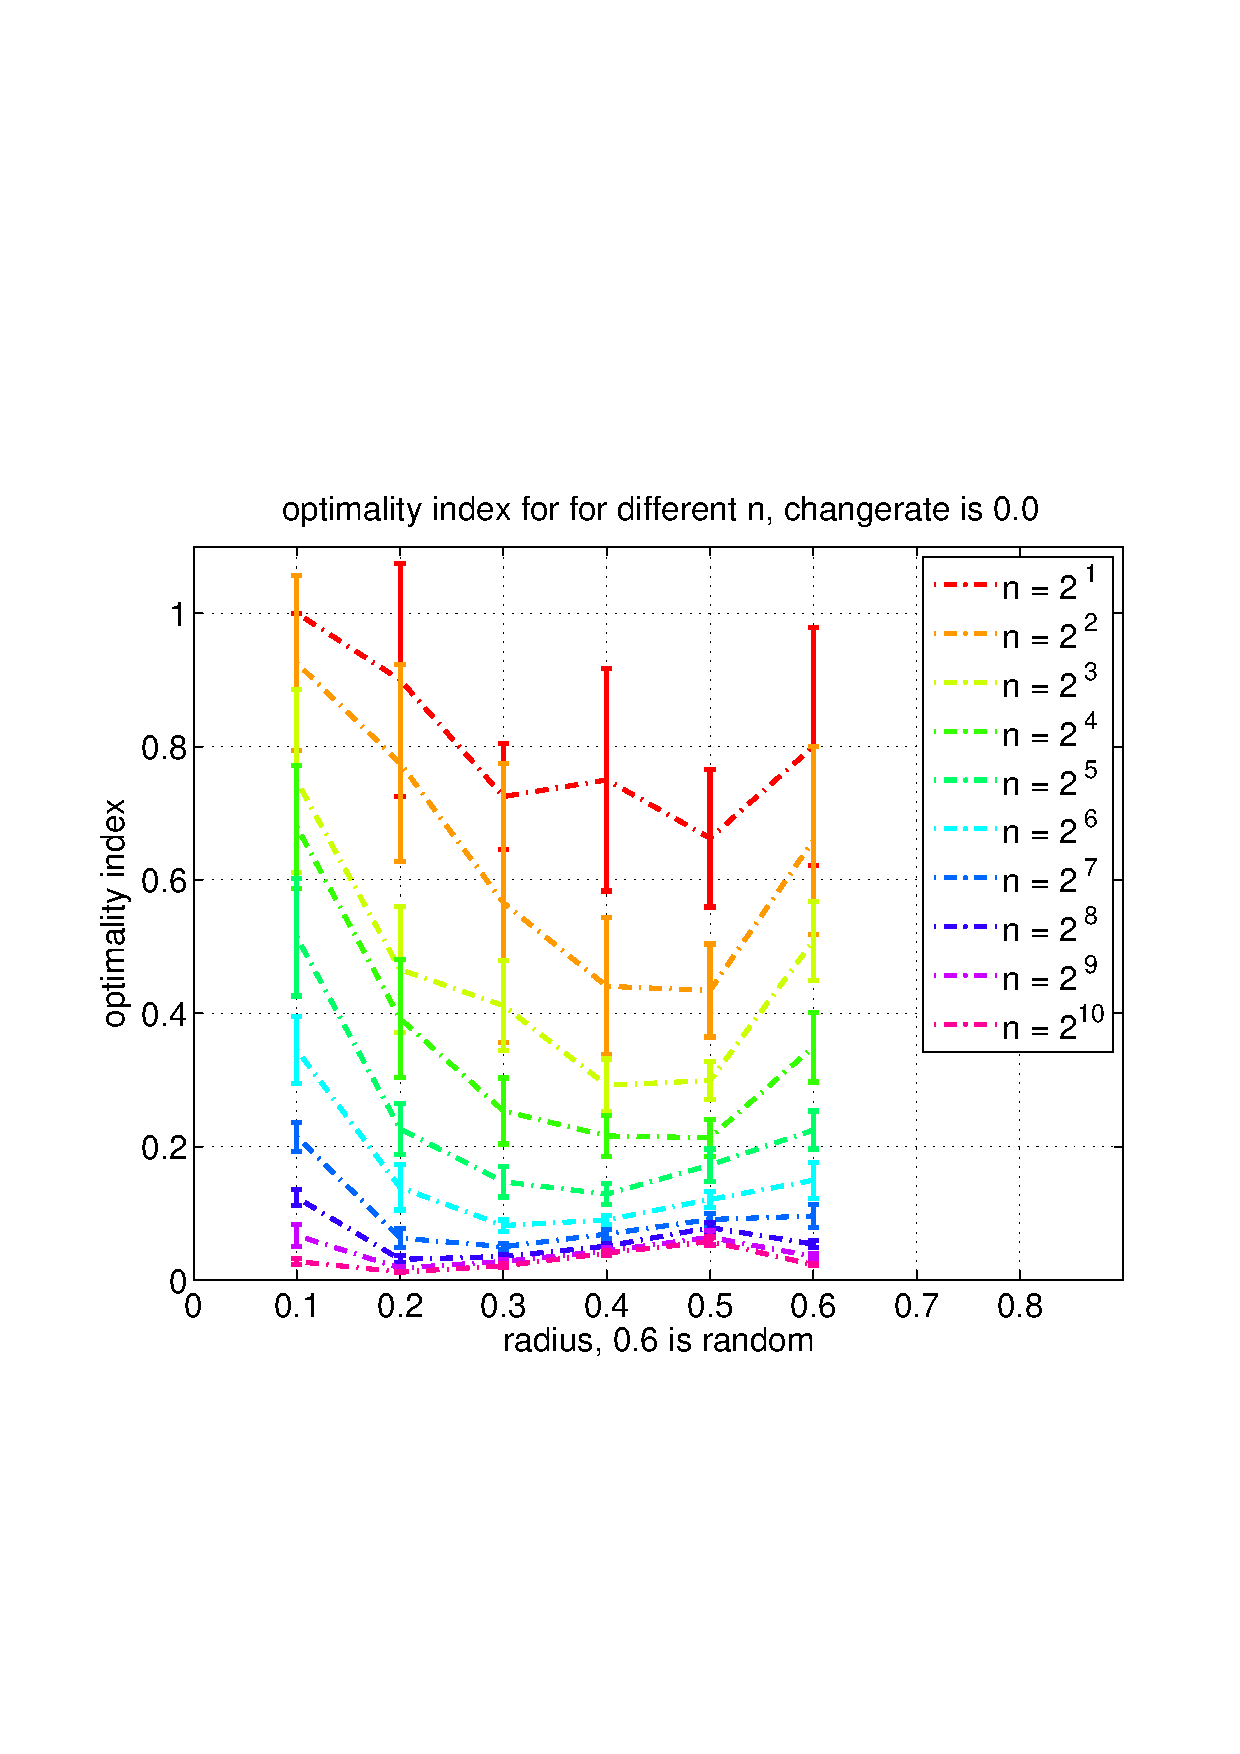
\includegraphics[trim=0 180 0 180, clip, height=8cm]{../../code/data/2014_12_12_00_55_41/figure_4}
	\caption{Errorbar plot for the optimality index in dependence of the visibility radius. The different lines correspond to different input
	sizes n. The preference change rate was set to 0.}
	\label{fig:optimality2}
\end{figure}

\subsubsection{Parameters}

The input parameters were chosen as follows: The input size is a power of 2. Due to the quadratic dependence of the \mcode{generatePlane}
algorithm, the highest power evaluated is $2^{10}=1024$. Originally we wanted to work with basis 10 but we had to change to basis 2 because
of performance reasons as well. For the visibility radius we took the discrete values \mcode{0.1:0.1:0.5}, and for the preference change rates
values in \mcode{0:0.5:1}. For each triple of parameters the simulation was performed 10 times.

\subsubsection{Effects of preference changes}

Surprisingly the expected effect of the preference changes could not be observed at all. The optimality index is about the same for the extreme
values 0 and 1 for the change rate, and also for 0.5. For small input sizes there is a small variation of the optimality index (that seems to be
caused more by random effects than an actual correltation). For higher n the plot lines are at constant height (see also section \ref{addplotopt}
in the Appendix for plots).

\subsection{Effects of visibility radius}

The results of the visibility radius variation do also not look very promising. In figure \ref{fig:optimality2} one can see that for low input sizes
(n = 2 to 32) there seems to be a dependence on the visibility radius, namely the optimality index decreases for higher visibility radii
(as we expected). But for higher n the effect disappears, and the optimality index even gets higher again for the visibility radius close to
0.5. Note that the points labeled with 0.6 on the x axis correspond to random radius and not visibility radius 0.6.

One way to explain this is that there might be several 'hidden' effects that cause this weird looking behavior. One of them could be that
the visibility radius is chosen to be constant for all input sizes. It is now not the same when thousand instead of only ten nodes are placed
in the plane, because for more nodes the number of nodes that happen to be in the neighborhood defined by a constant visibility radius is much
higher.

\subsection{Input size dependency}
\comment{
\begin{figure}[h!]
	\begin{subfigure}[b]{\textwidth}
	  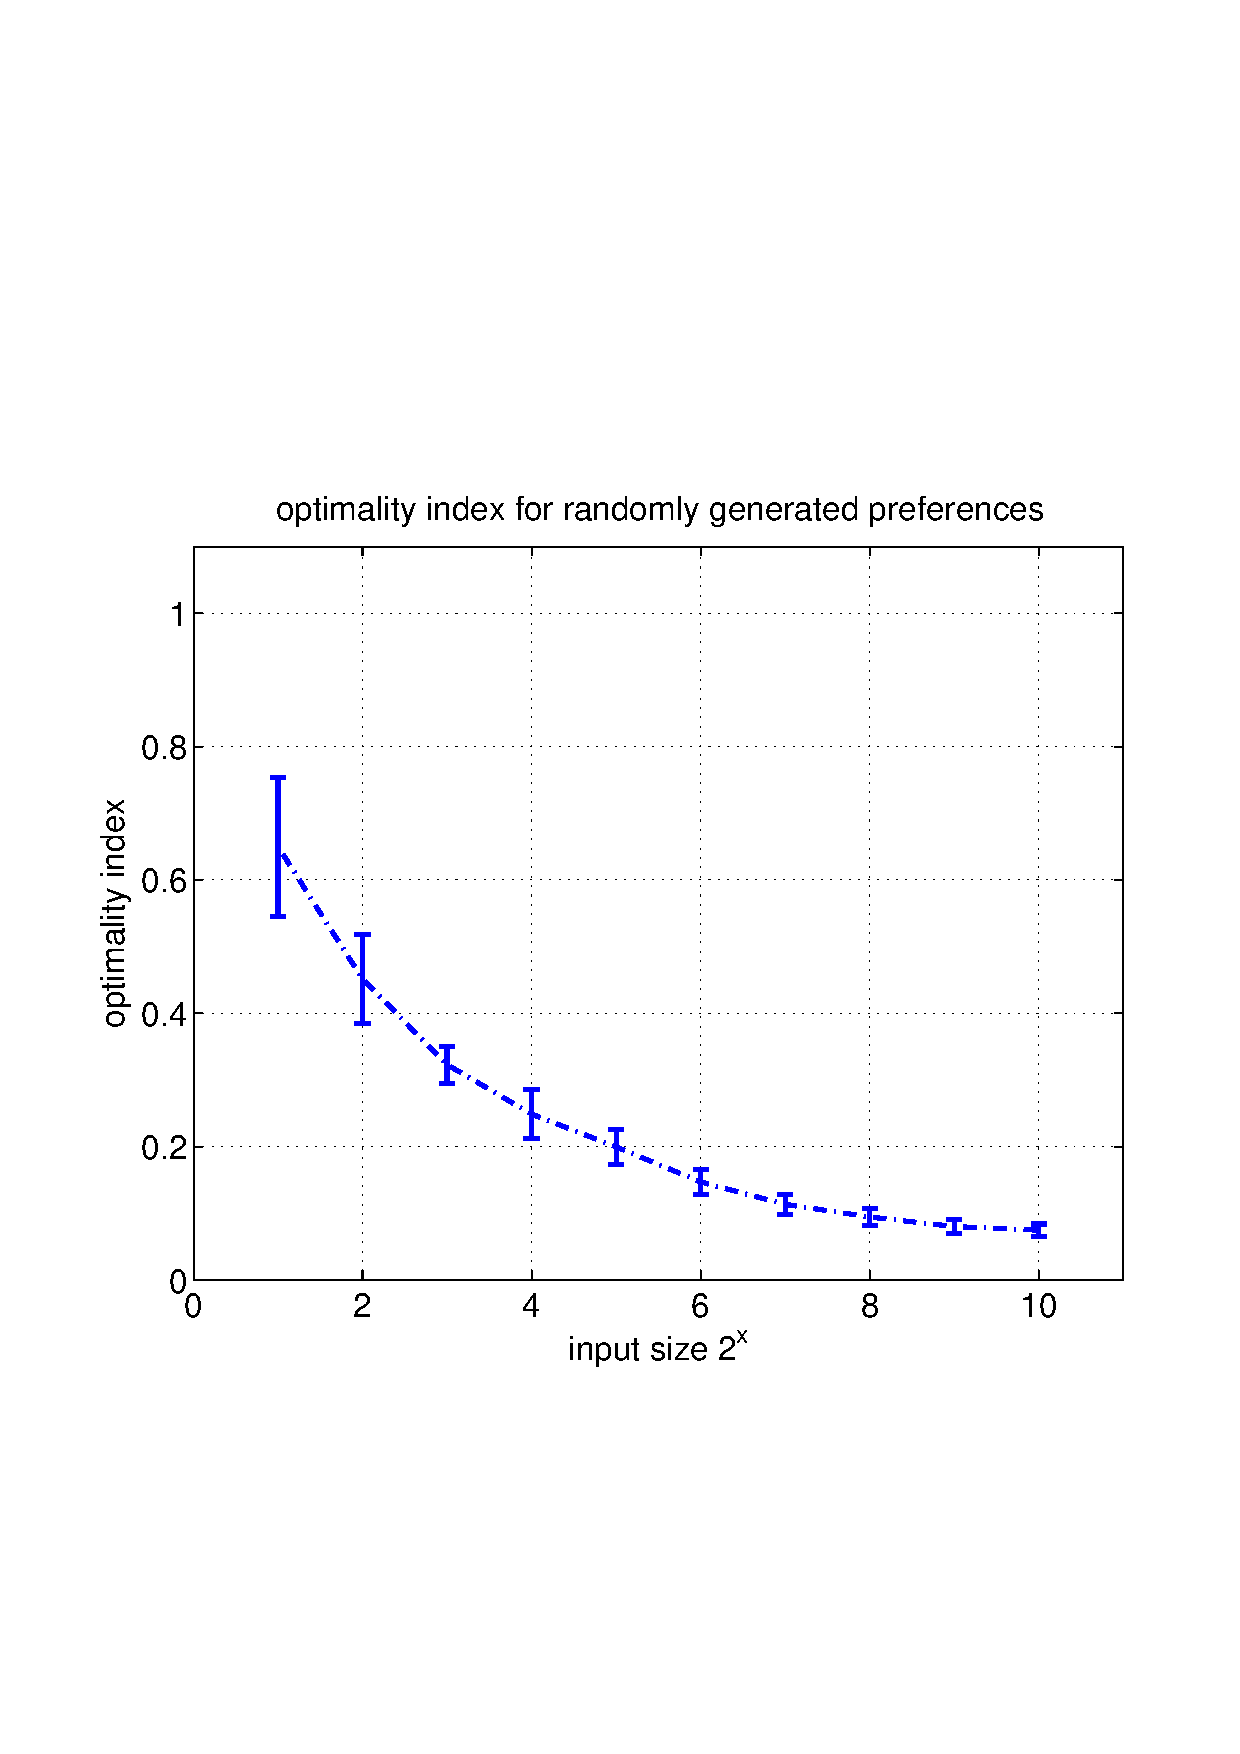
\includegraphics[trim=0 180 0 180, clip, height=10cm]{../../code/data/2014_12_12_00_55_41/figure_14}
	  \caption{Preferences generated randomly}
	  \label{fig:optimality1a}
	\end{subfigure}
  \begin{subfigure}[b]{\textwidth}
	  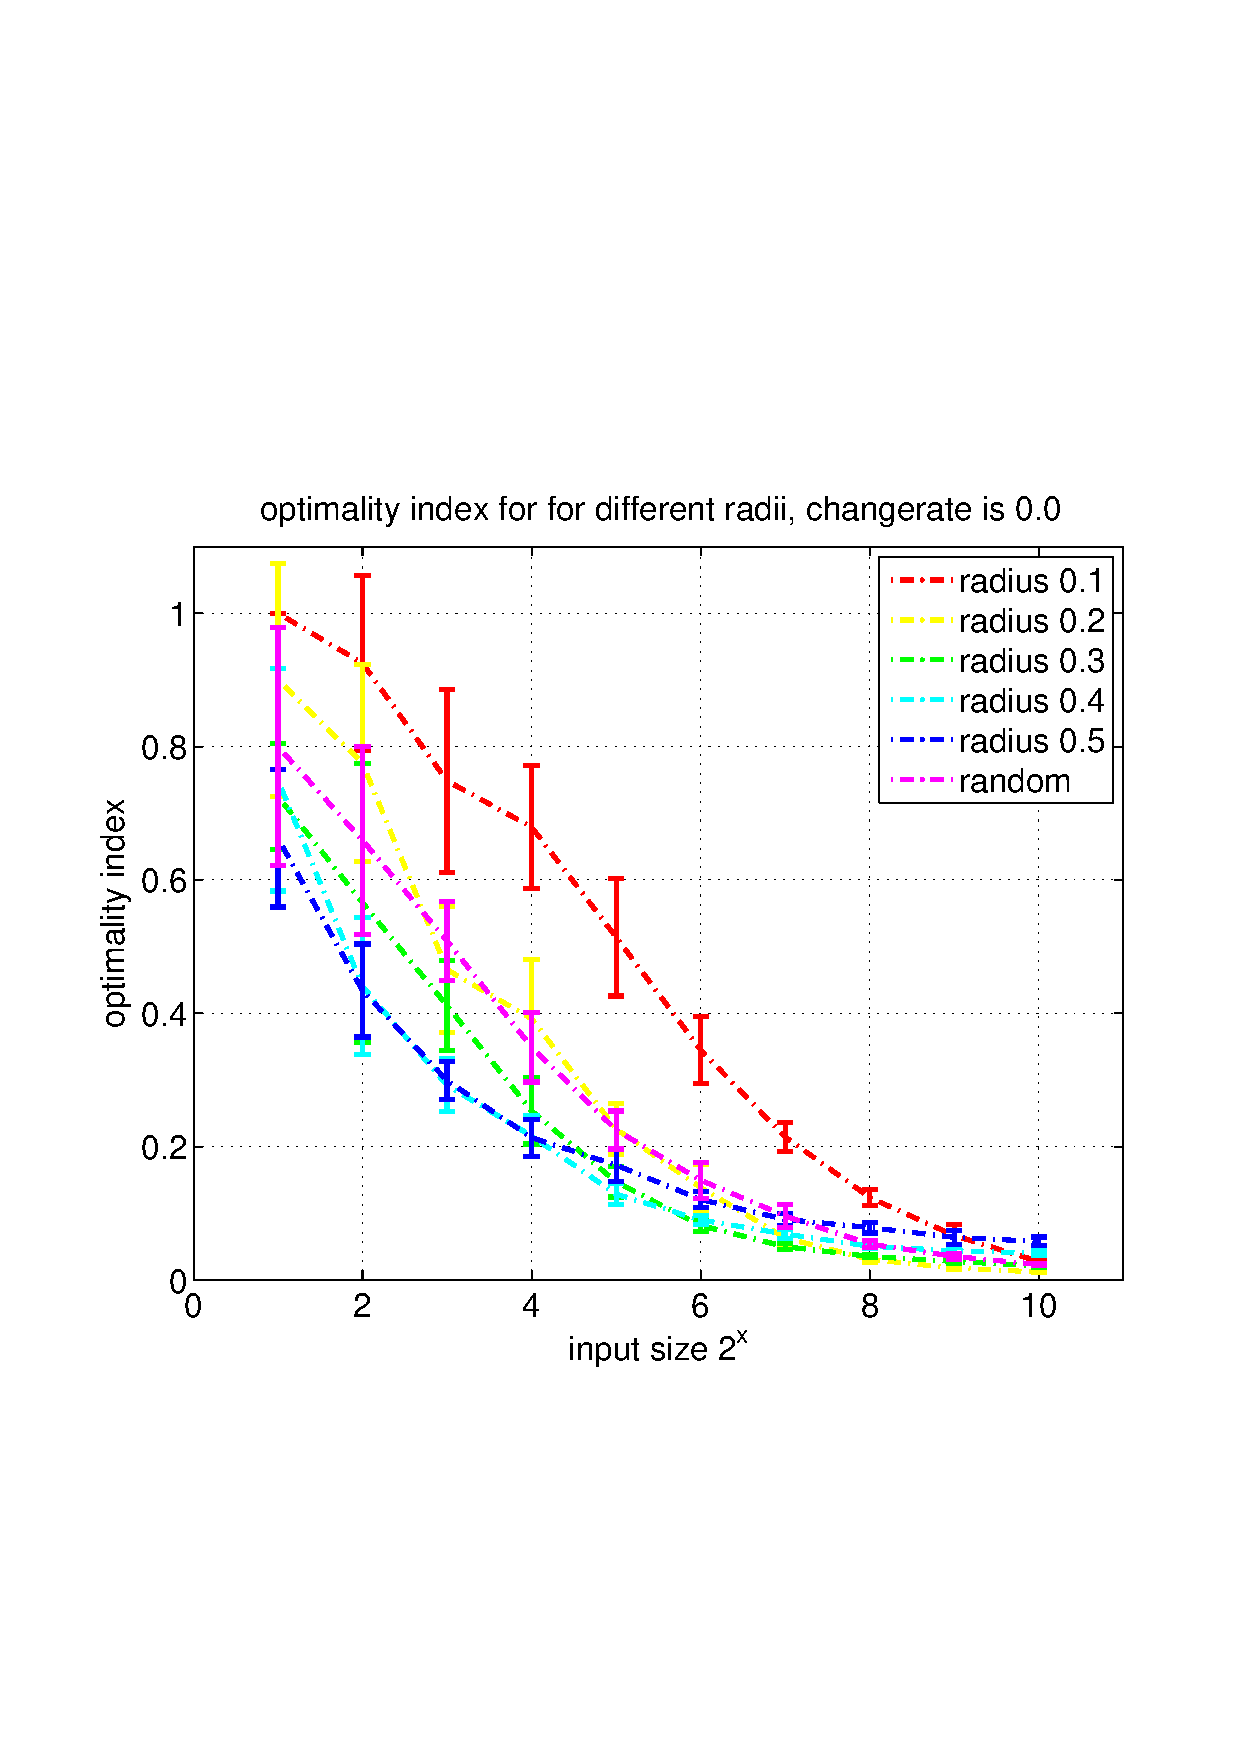
\includegraphics[trim=0 180 0 180, clip, height=10cm]{../../code/data/2014_12_12_00_55_41/figure_1}
	  \caption{Preferences generated by the \mcode{generatePlane} algorithm. Different lines represent different visibility radii.}
	  \label{fig:optimality1b}
	\end{subfigure}
	\caption{Optimality index errorbar plot in dependence of input size n}
	\label{fig:optimality1}
\end{figure}}

\begin{figure}[h]
  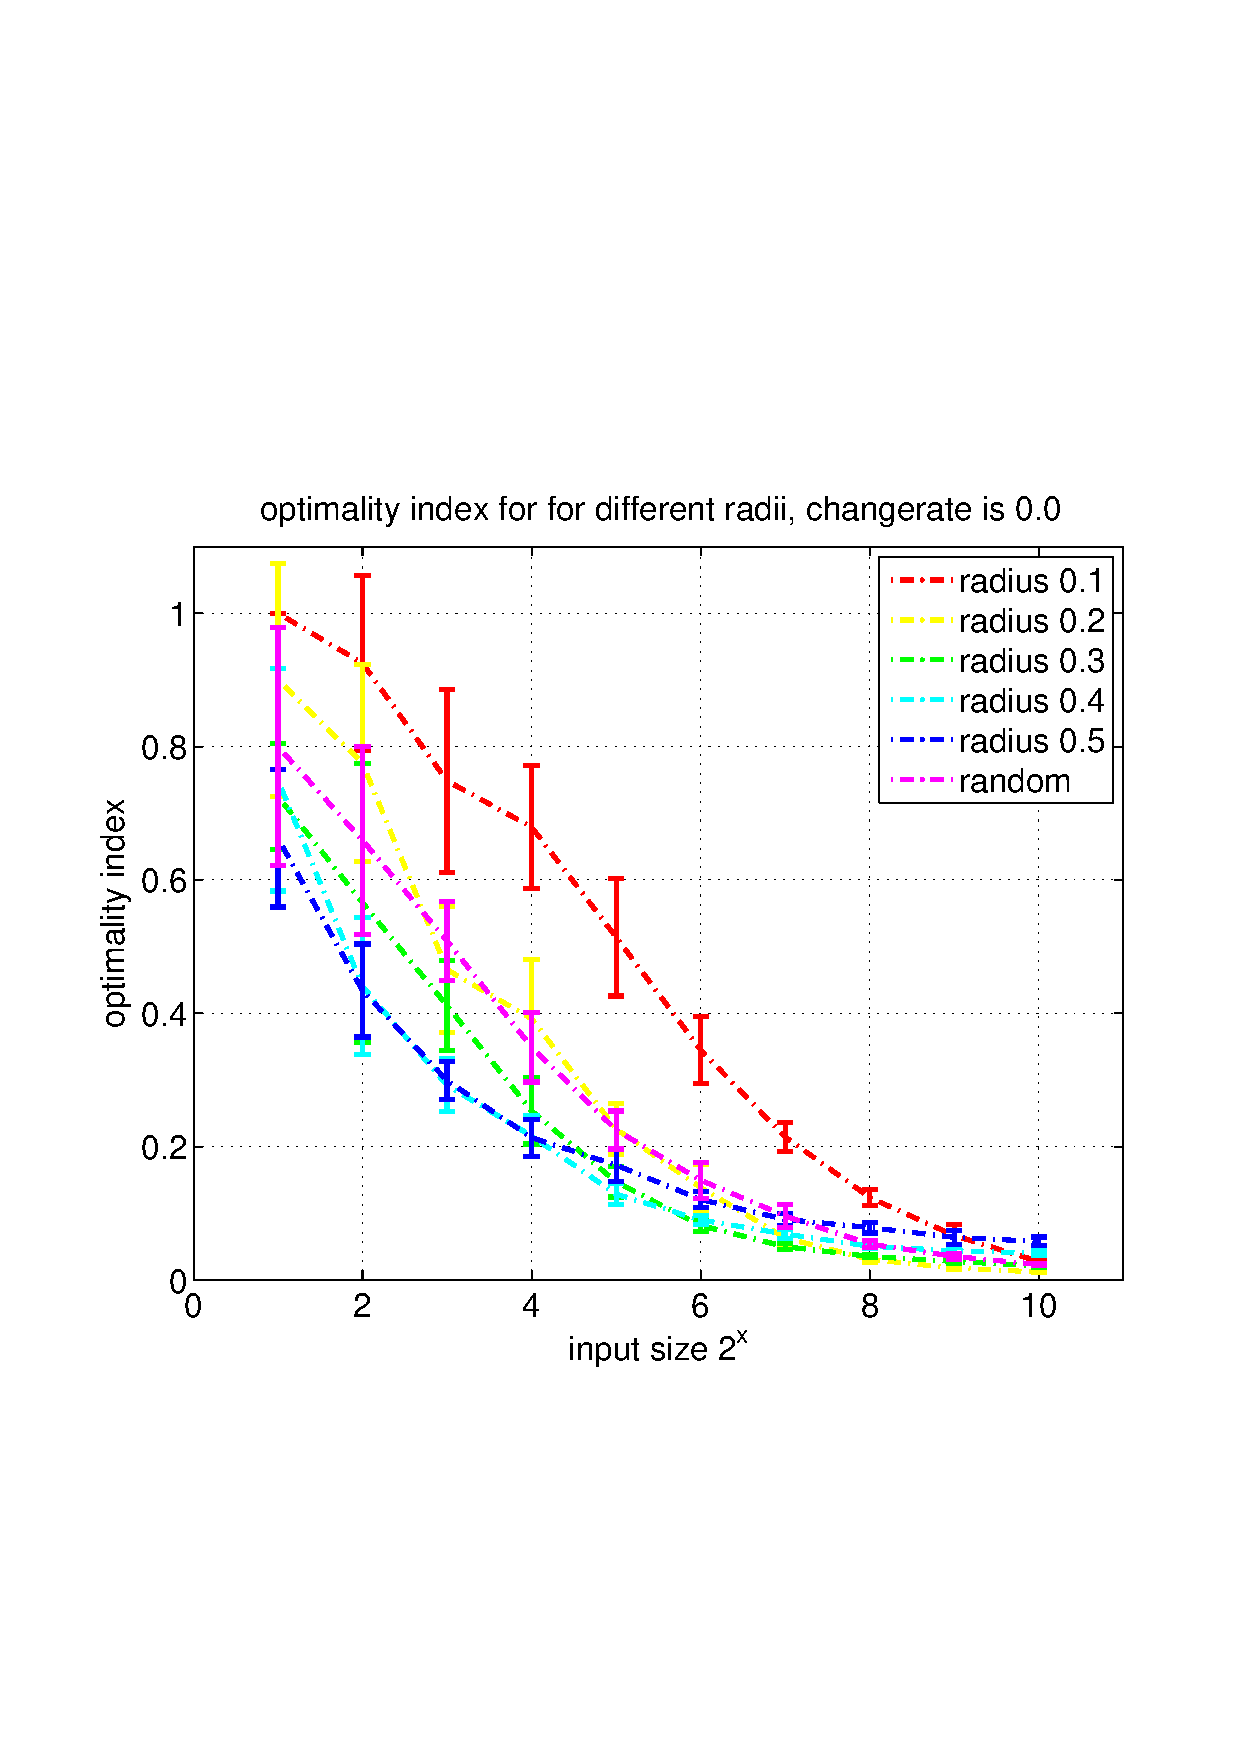
\includegraphics[trim=0 180 0 180, clip, height=8cm]{../../code/data/2014_12_12_00_55_41/figure_1}
  \caption{Optimality index errorbar plot in dependence of input size n. Preferences were generated by the \mcode{generatePlane} algorithm. Different lines represent different visibility radii.}
  \label{fig:optimality1a}
\end{figure}
\begin{figure}[h]
  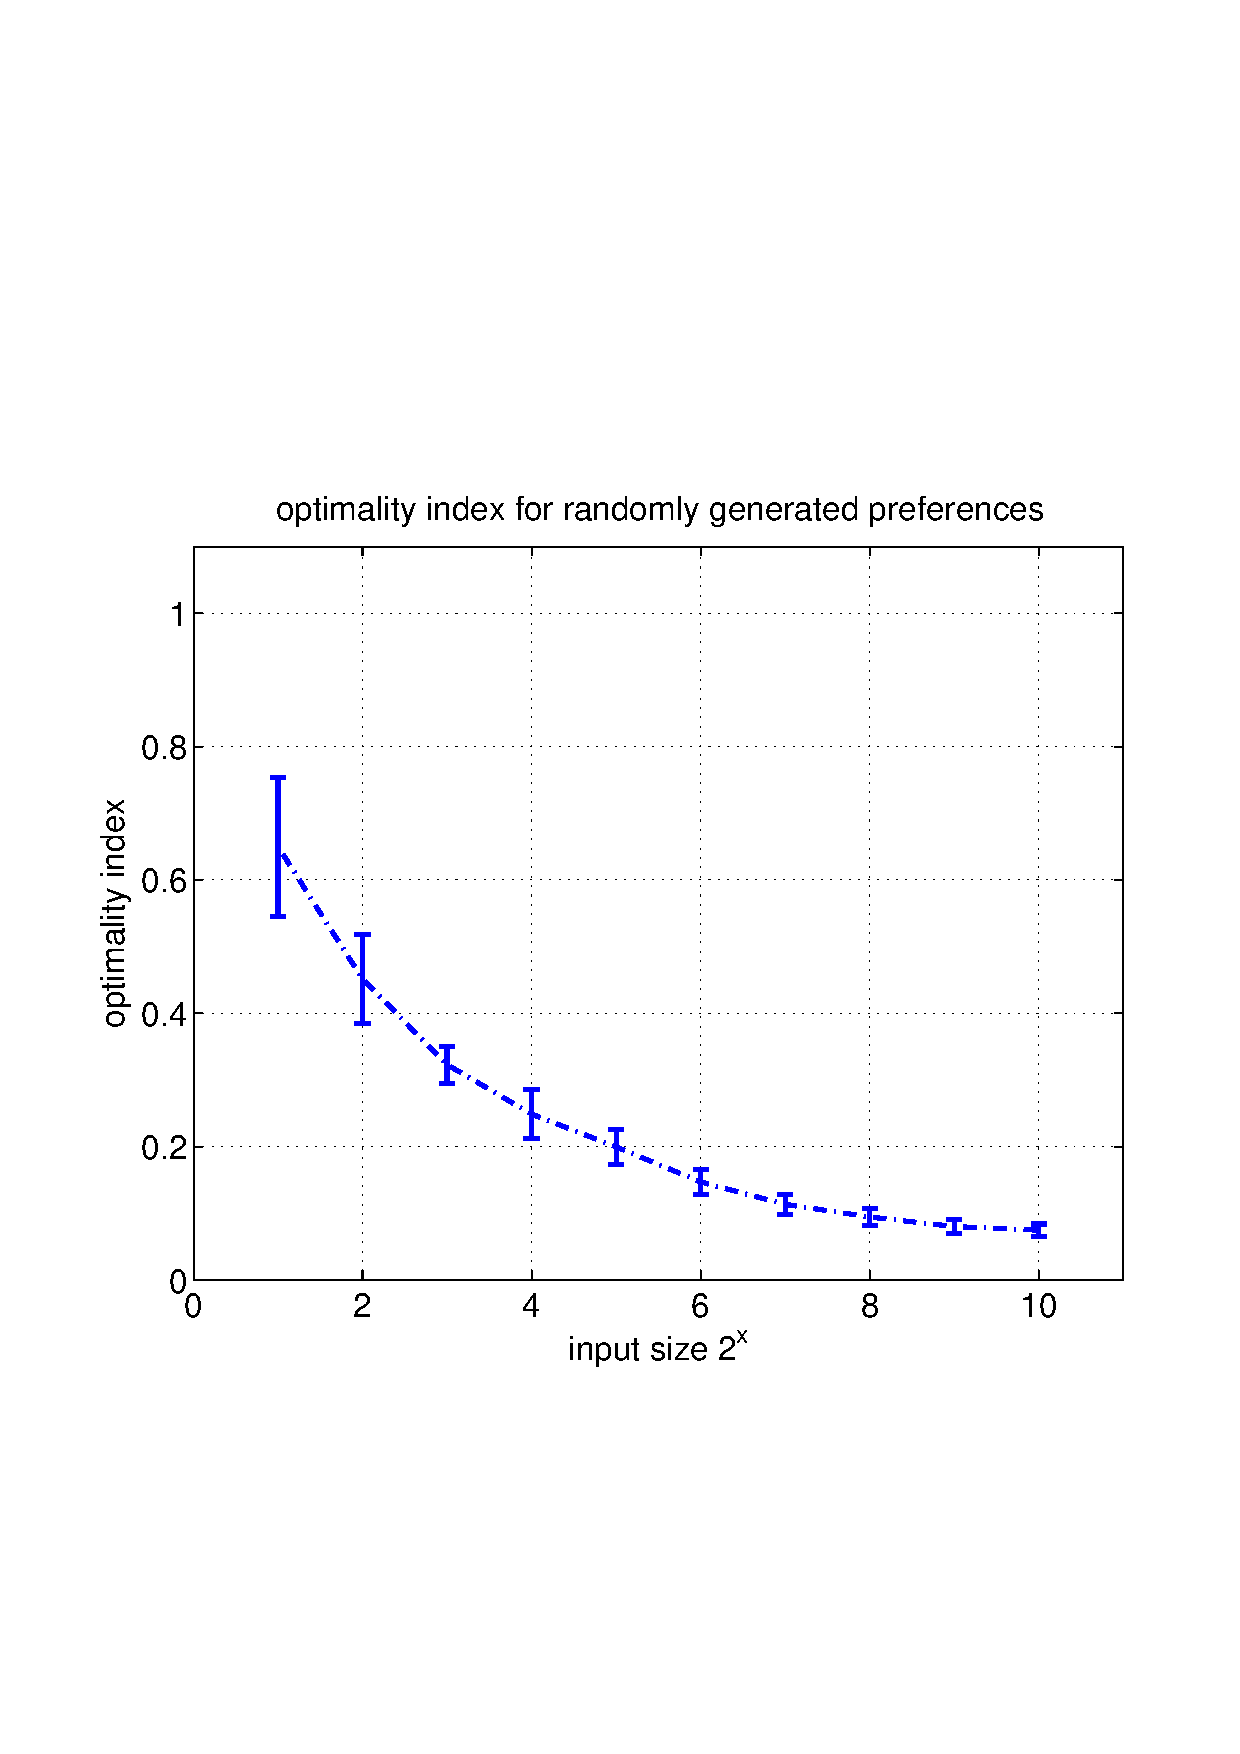
\includegraphics[trim=0 180 0 180, clip, height=8cm]{../../code/data/2014_12_12_00_55_41/figure_14}
  \caption{Optimality index errorbar plot in dependence of input size n. Preferences were generated randomly.}
  \label{fig:optimality1b}
\end{figure}

Looking at figure \ref{fig:optimality1a}, one can clearly observe that the optimality index gets smaller for increasing input size, meaning that
the result is more optimal for higher n. This is a bit counterintuitive at first thought. Why should the result be less optimal for smaller n?
One could think that this effect is somehow produced by the modifications that were made to the Gale-Shapley algorithm. But it turns
out that the effect can also be observed for randomly generated preference lists using \mcode{generateRandom}, see figure \ref{fig:optimality1b}.
For this type of preference lists none of the 'special treatments' in the modified algorithm (e. g. empty preference lists) apply, but the
effect can still be observed.



\newpage
\section{Summary and Outlook}

\renewcommand{\refname}{\section{References}}

\bibliographystyle{plainnat}
\bibliography{references}

% jstor pdf link http://www.jstor.org/stable/pdfplus/2312726.pdf

\section{Appendix A: MATLAB Codes}

\subsection*{generateRandom.m}
\lstinputlisting{../../code/generateRandom.m}
\subsection*{generatePlane.m}
\lstinputlisting{../../code/generatePlane.m}
\subsection*{vprintf.m}
\lstinputlisting{../../code/vprintf.m}
\subsection*{makeMatch.m}
\lstinputlisting{../../code/makeMatch.m}
\subsection*{checkEngagements.m}
\lstinputlisting{../../code/checkEngagements.m}
\subsection*{simulation.m}
\lstinputlisting{../../code/simulation.m}
\subsection*{simulation2.m}
\lstinputlisting{../../code/simulation2.m}
\subsection*{simulation3.m}
\lstinputlisting{../../code/simulation3.m}
\subsection*{iteratesimulation.m}
\lstinputlisting{../../code/iteratesimulation.m}
\subsection*{plot3.m}
\lstinputlisting{../../code/plot3.m}

\newpage
\section{Appendix B: Plots}

Additional Plots

\subsection{Optimality Index} \label{addplotopt}

\begin{figure}[h!]
	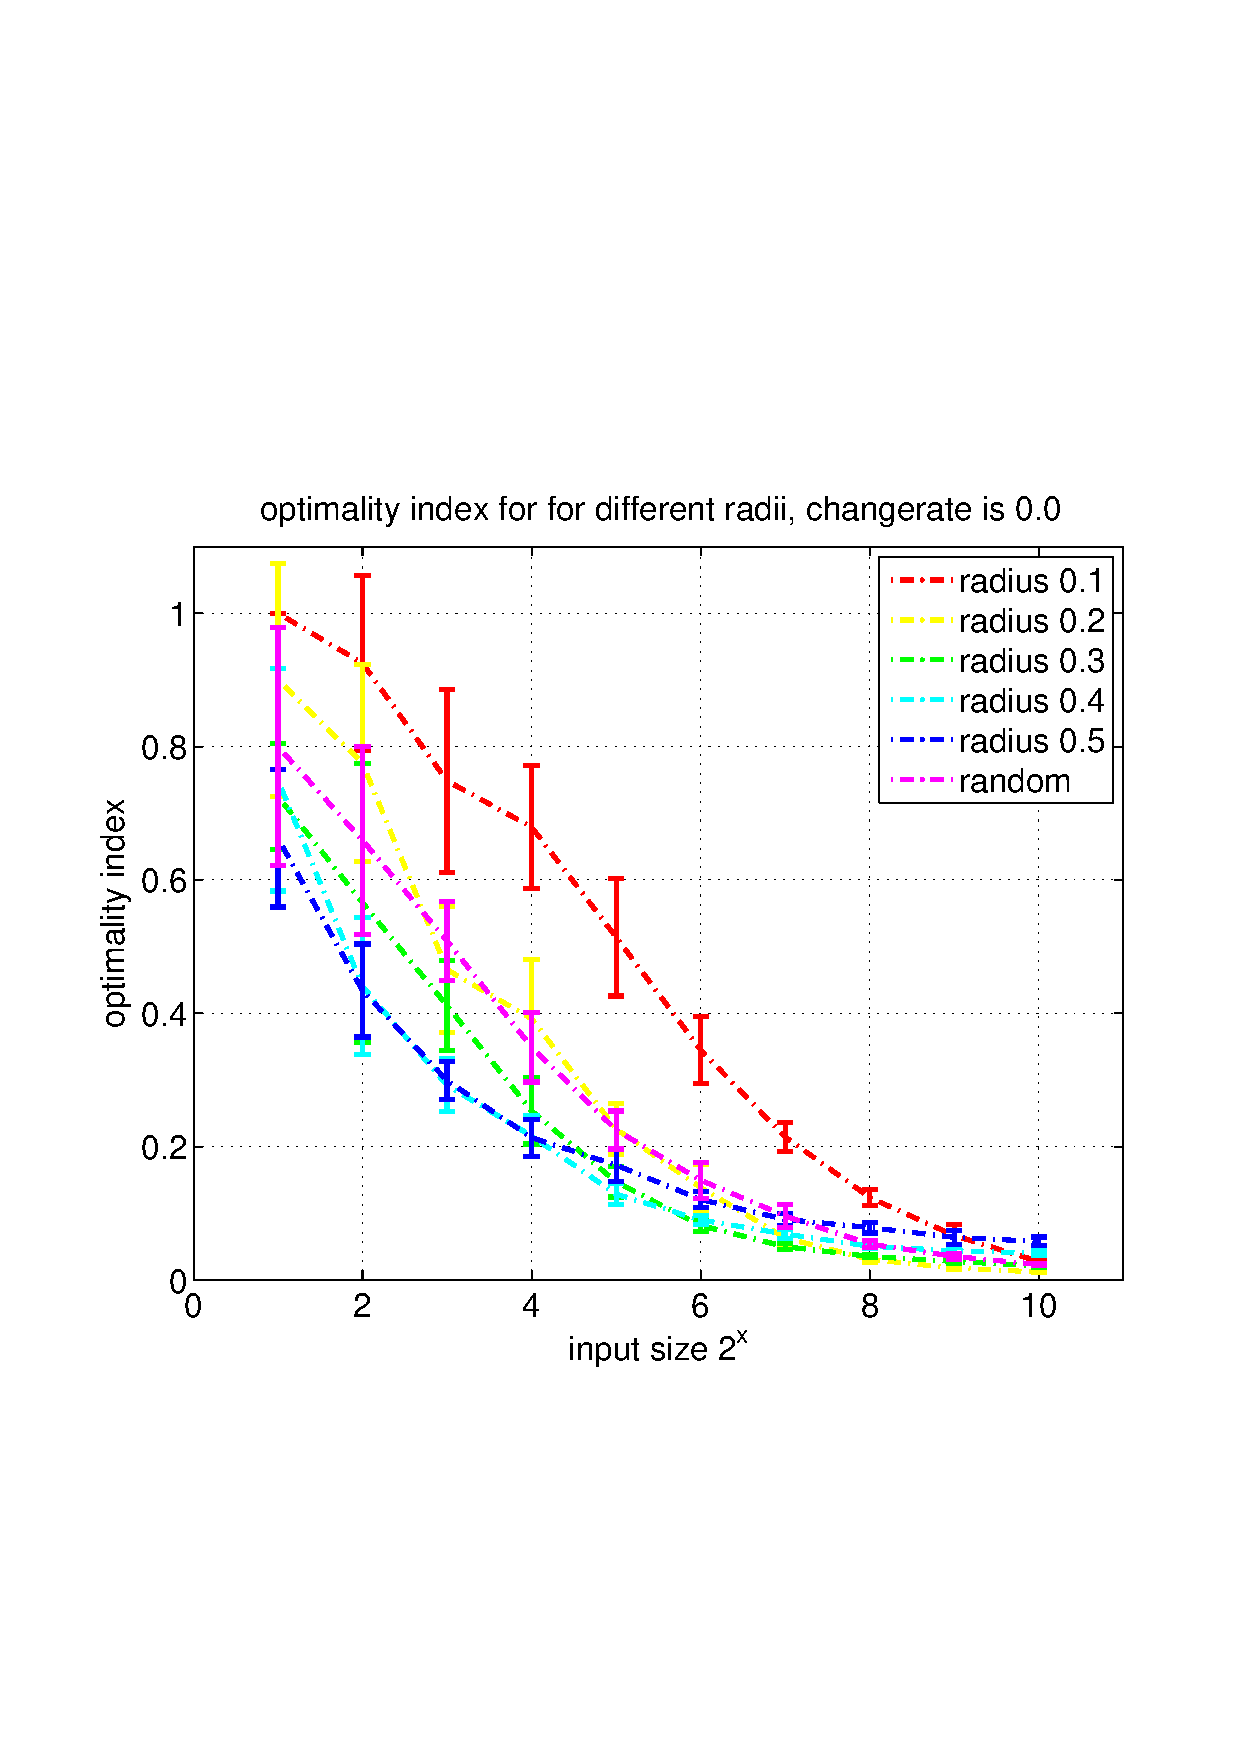
\includegraphics[trim=0 180 0 180, clip,width=\linewidth]{../../code/data/2014_12_12_00_55_41/figure_1}
\end{figure}
\begin{figure}
	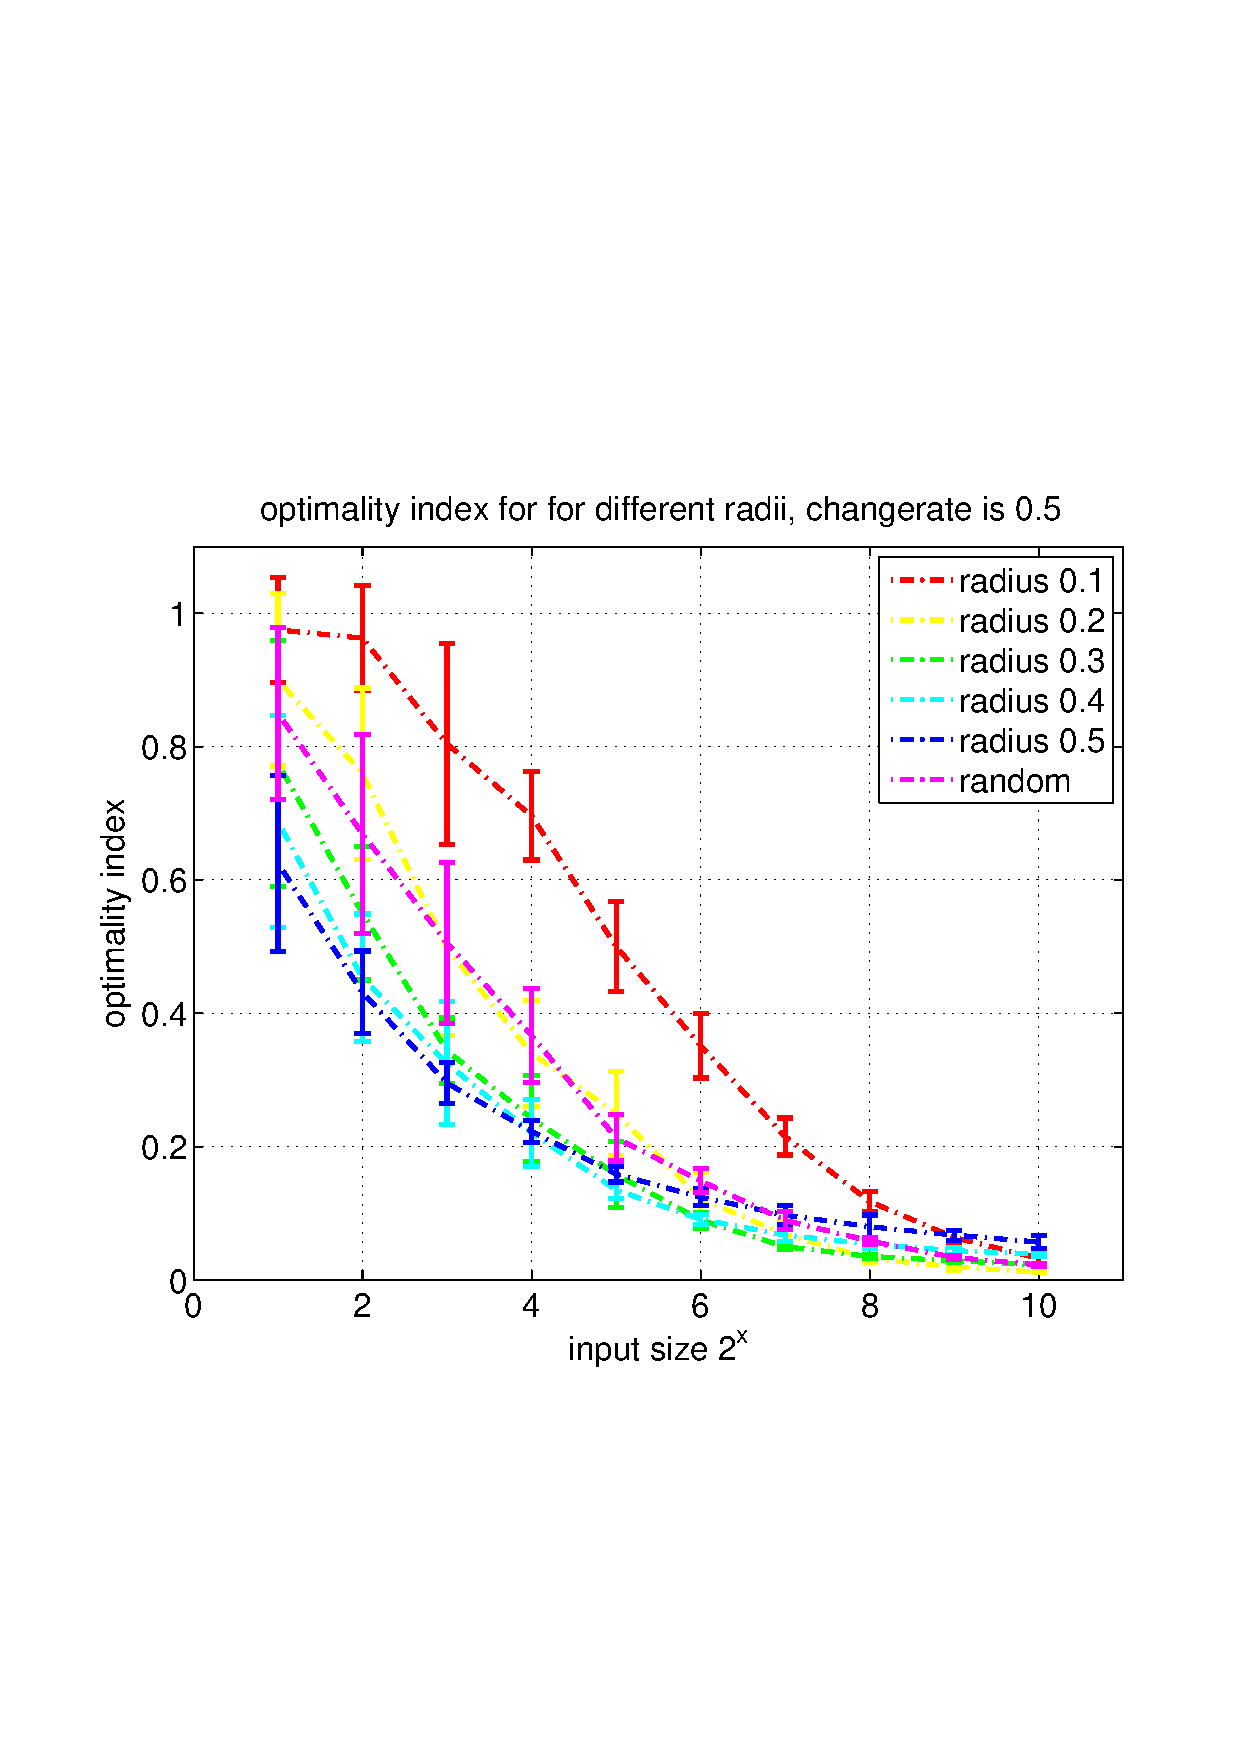
\includegraphics[width=\linewidth]{../../code/data/2014_12_12_00_55_41/figure_2}
\end{figure}
\begin{figure}
	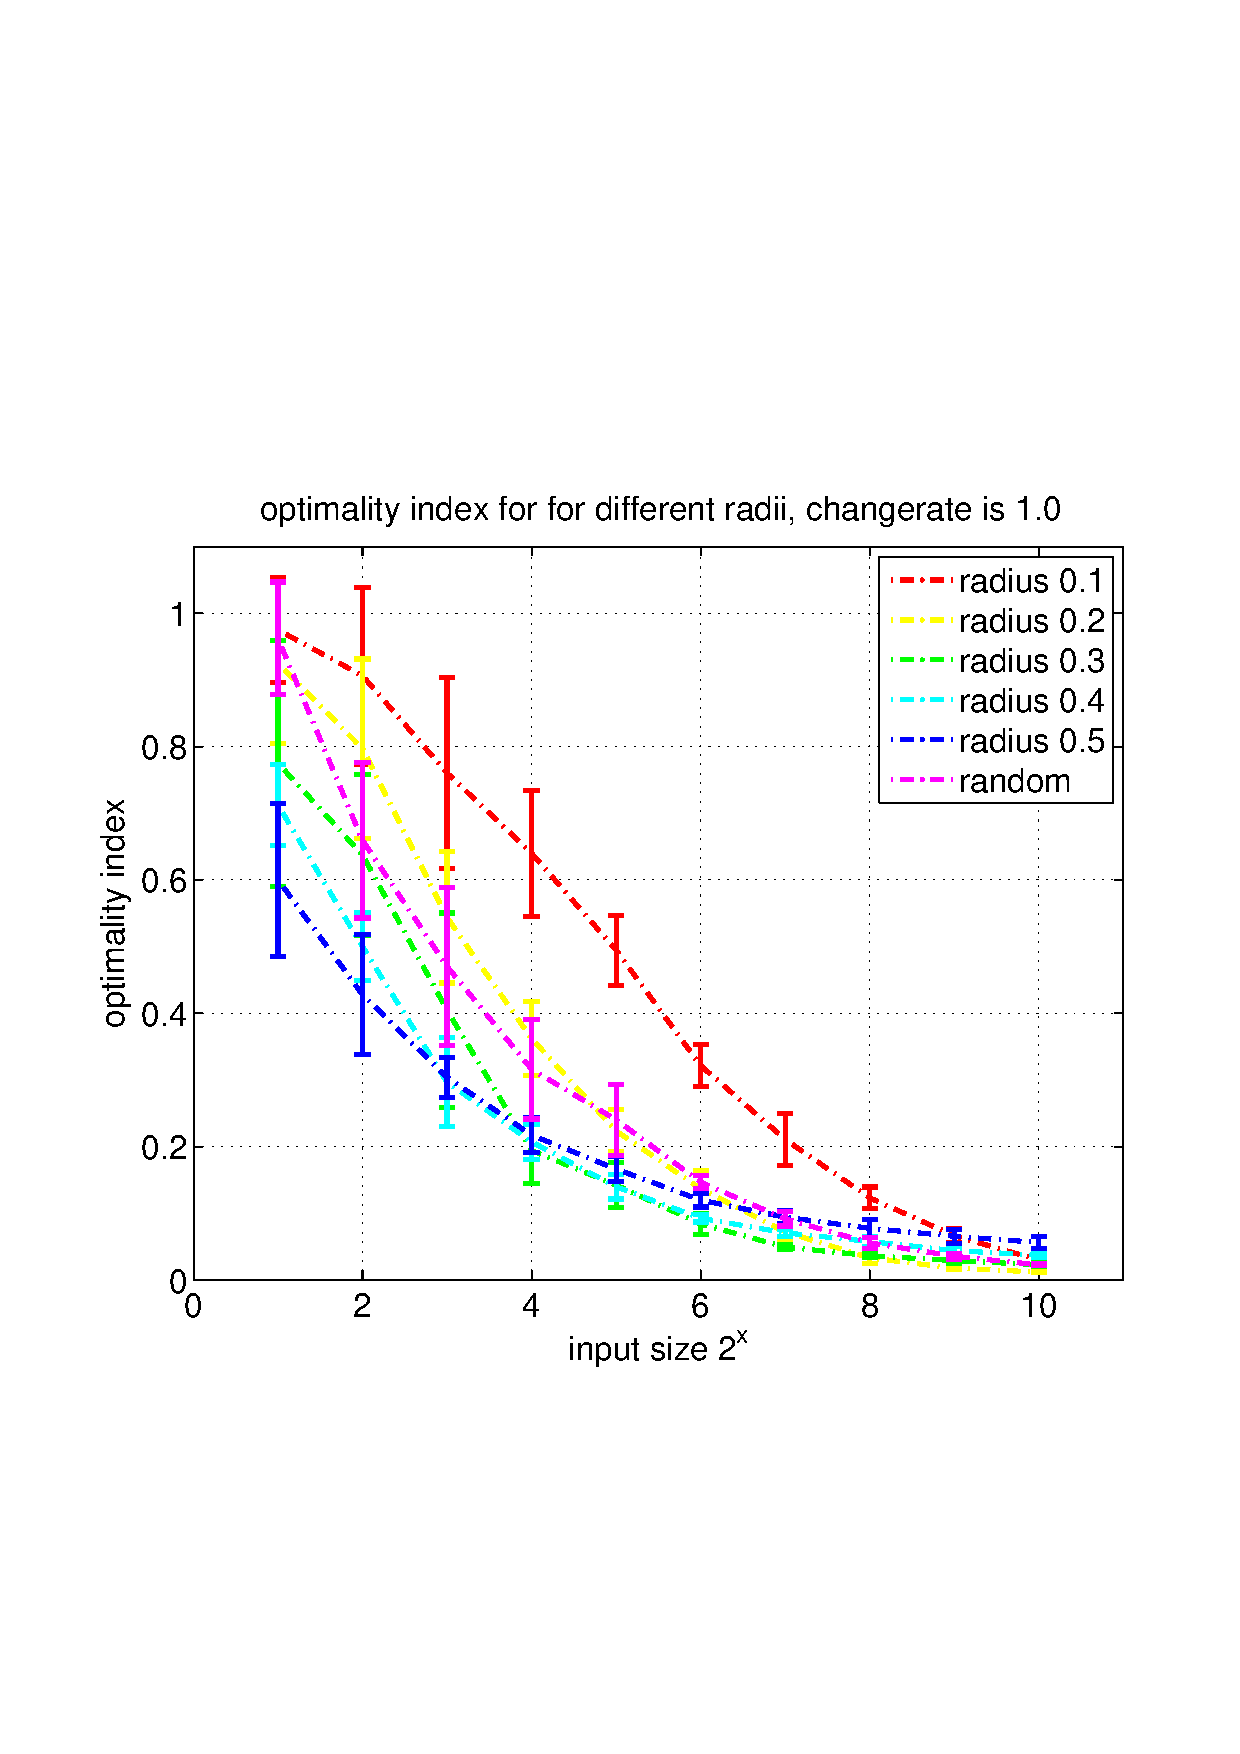
\includegraphics[width=\linewidth]{../../code/data/2014_12_12_00_55_41/figure_3}
\end{figure}
\begin{figure}
	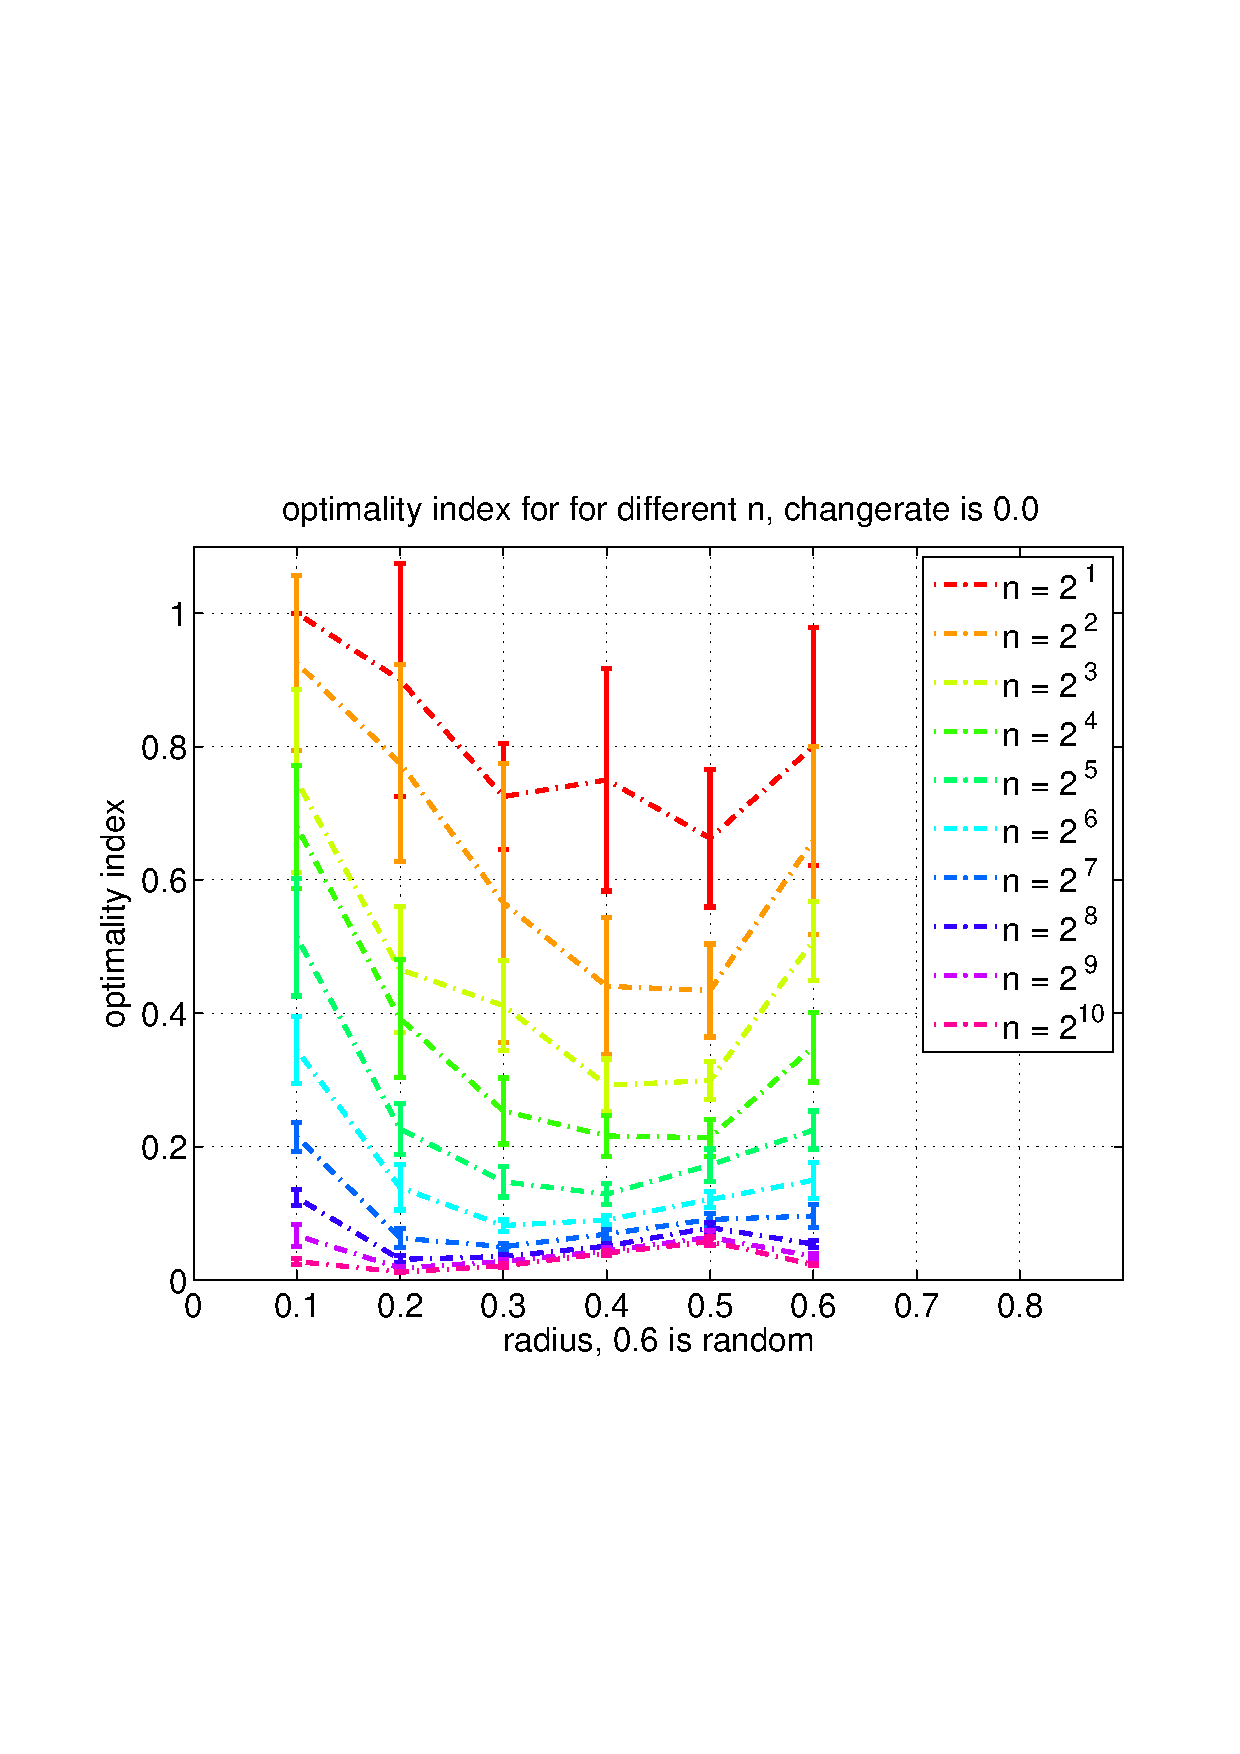
\includegraphics[width=\linewidth]{../../code/data/2014_12_12_00_55_41/figure_4}
\end{figure}
\begin{figure}
	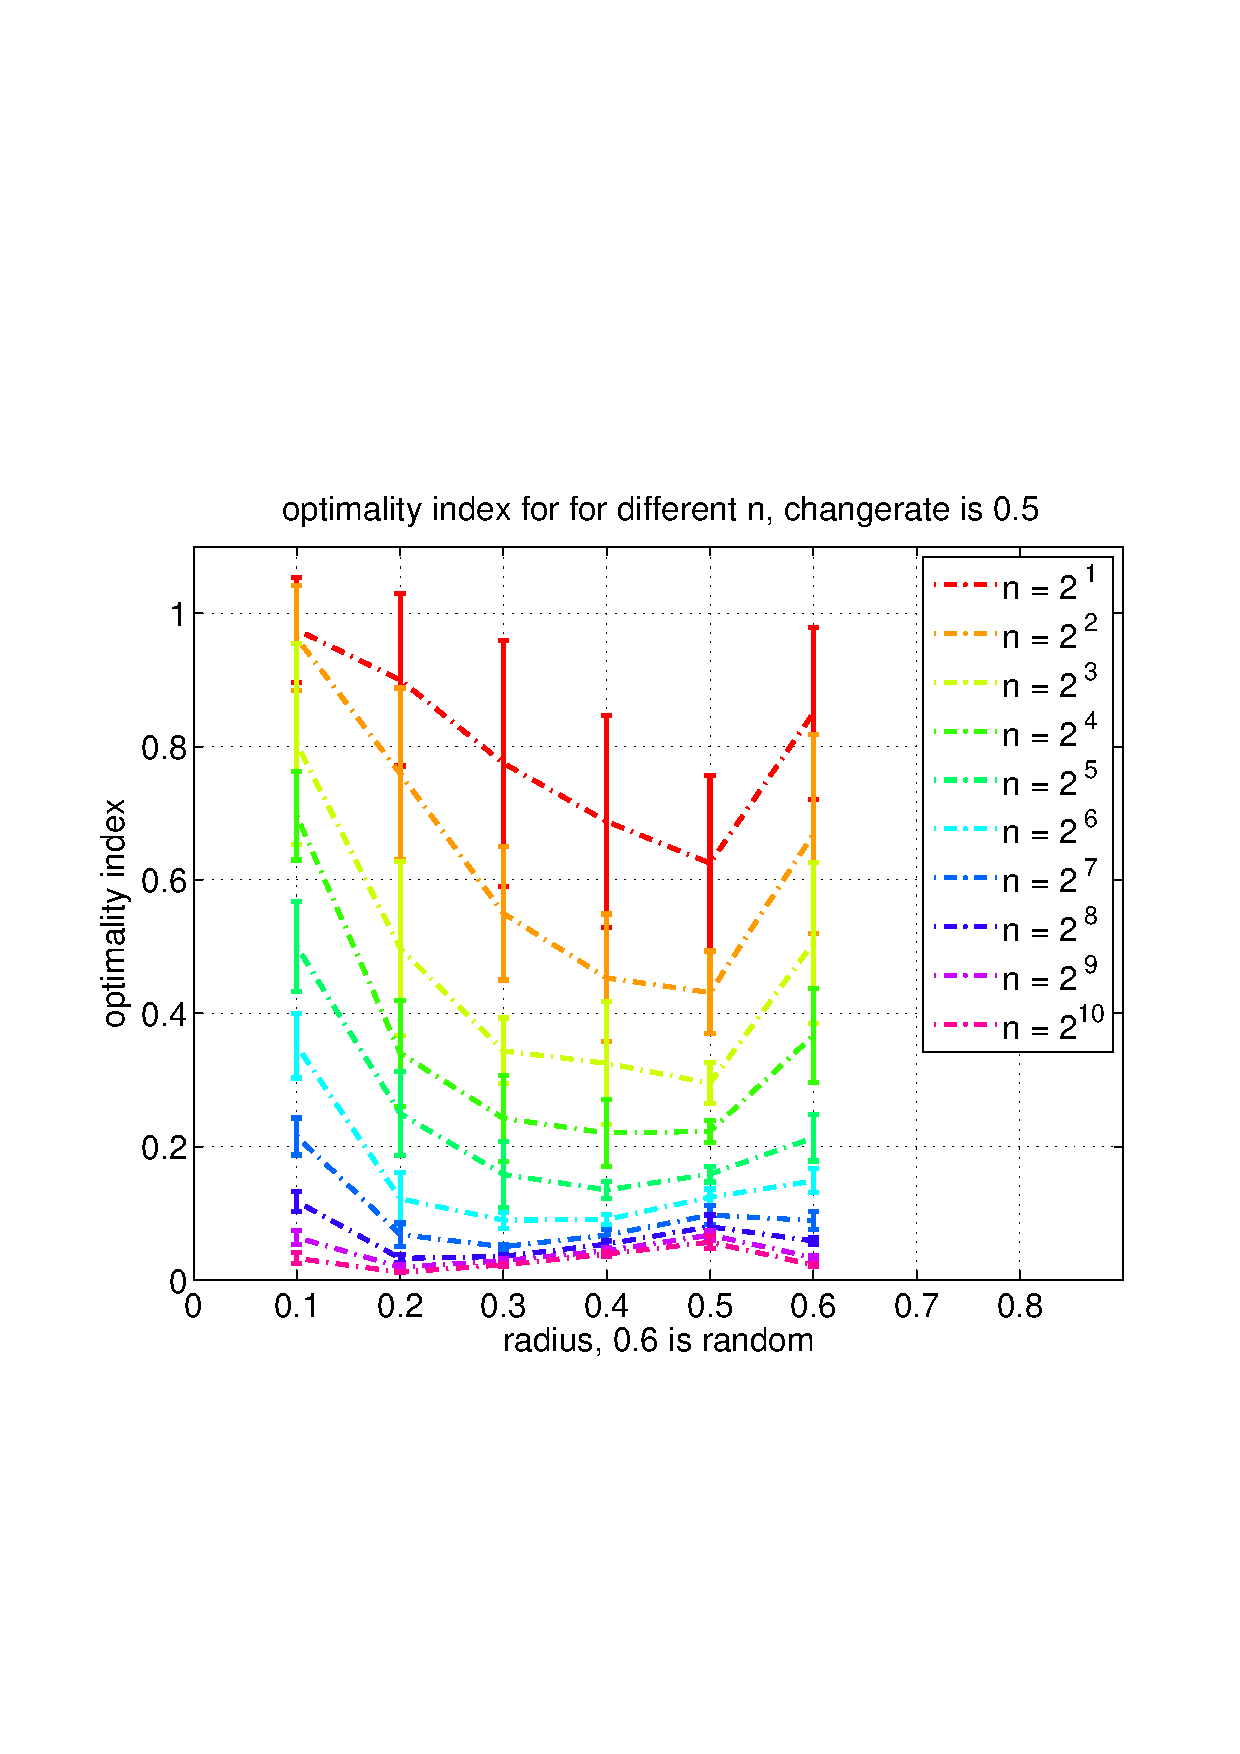
\includegraphics[width=\linewidth]{../../code/data/2014_12_12_00_55_41/figure_5}
\end{figure}
\begin{figure}
	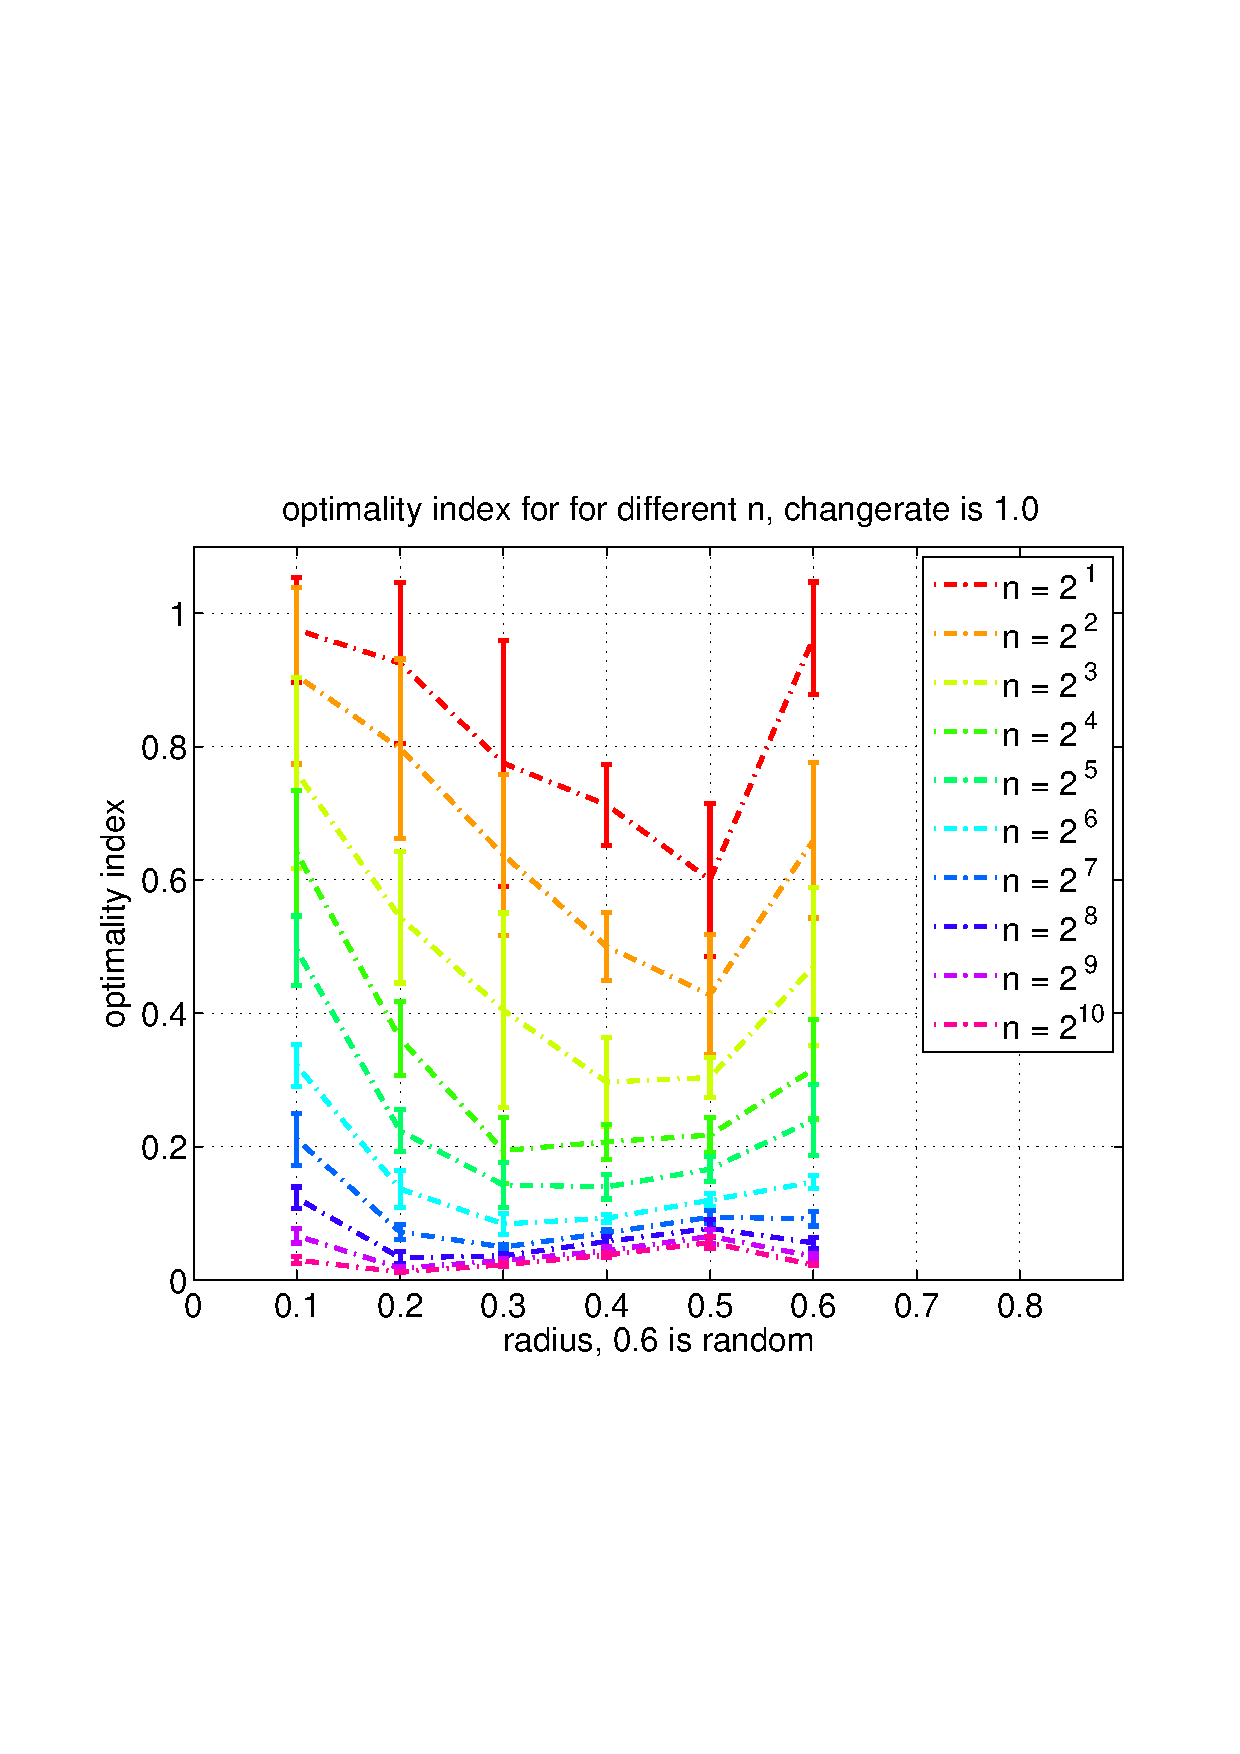
\includegraphics[width=\linewidth]{../../code/data/2014_12_12_00_55_41/figure_6}
\end{figure}
\begin{figure}
	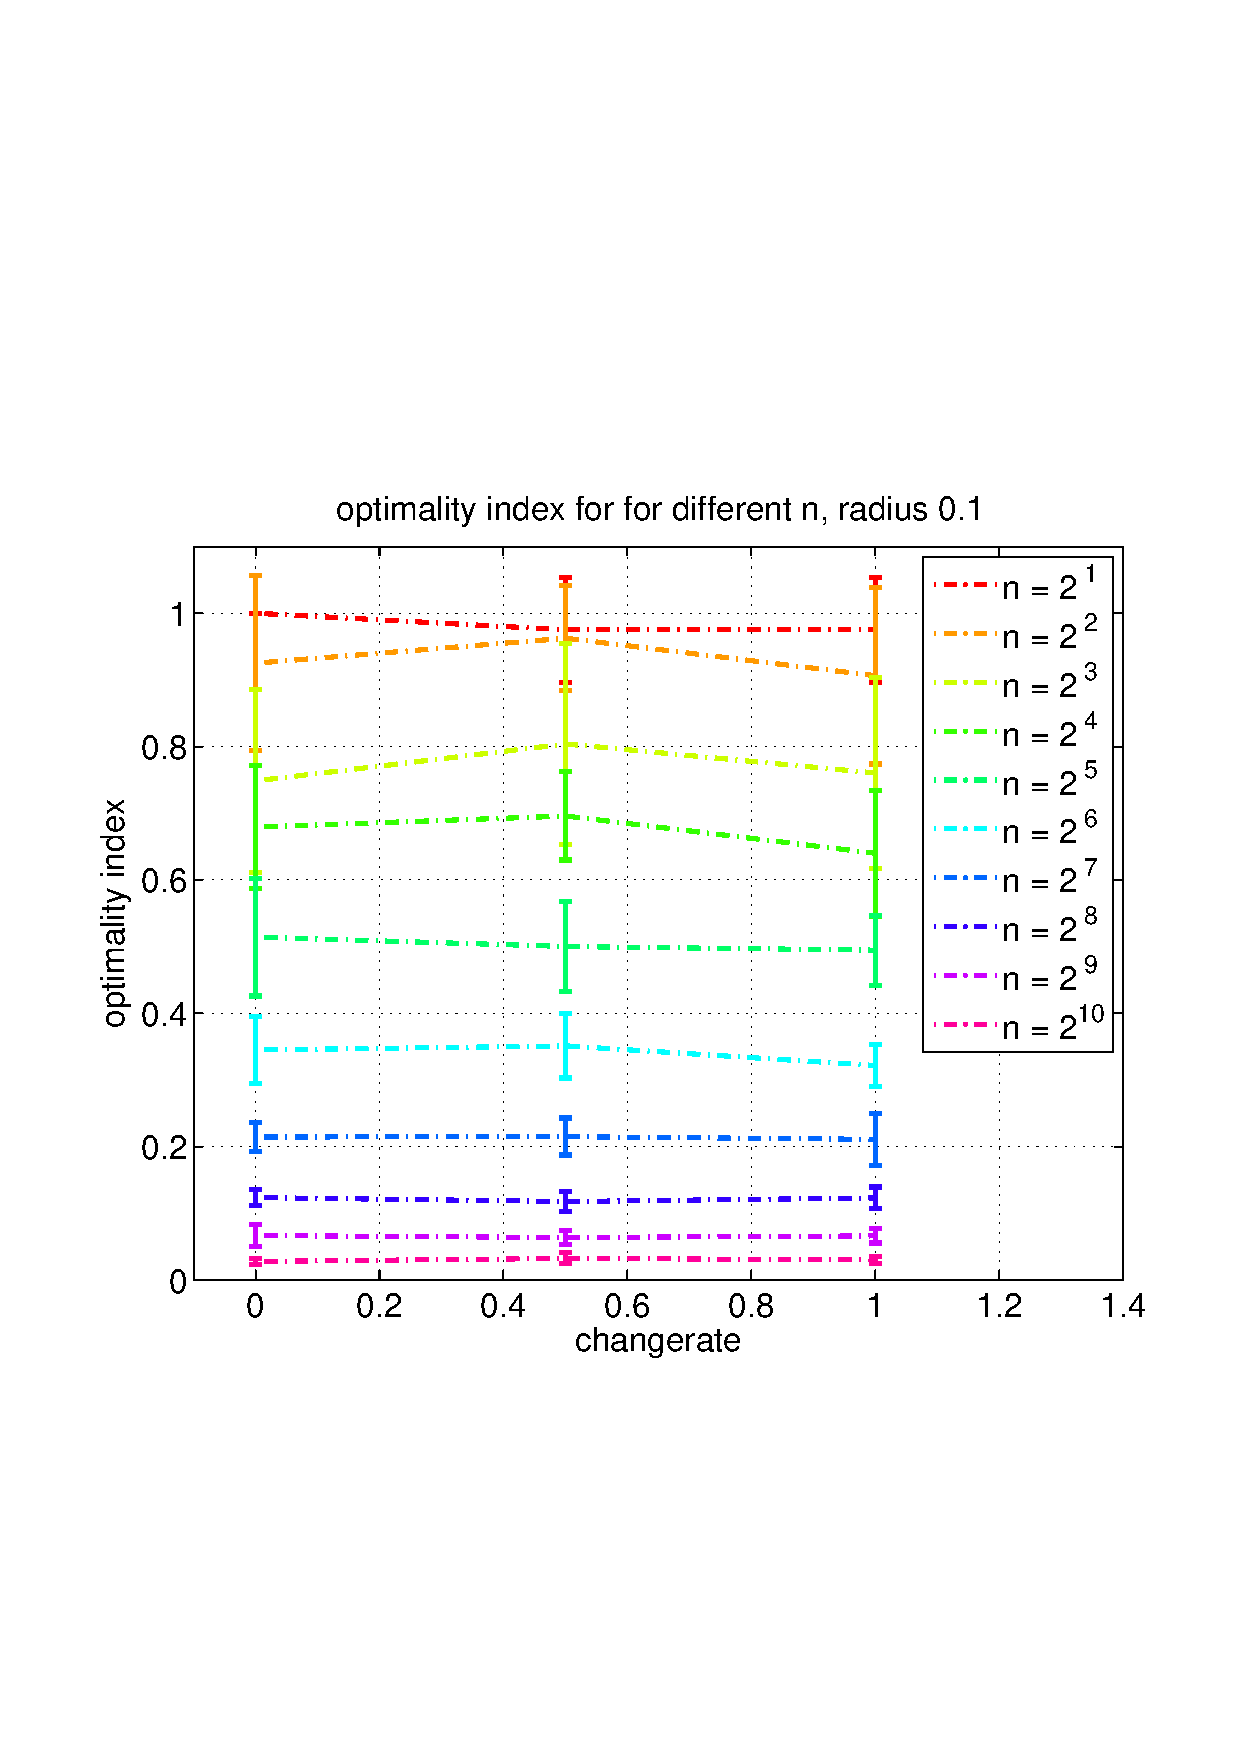
\includegraphics[width=\linewidth]{../../code/data/2014_12_12_00_55_41/figure_7}
\end{figure}
\begin{figure}
	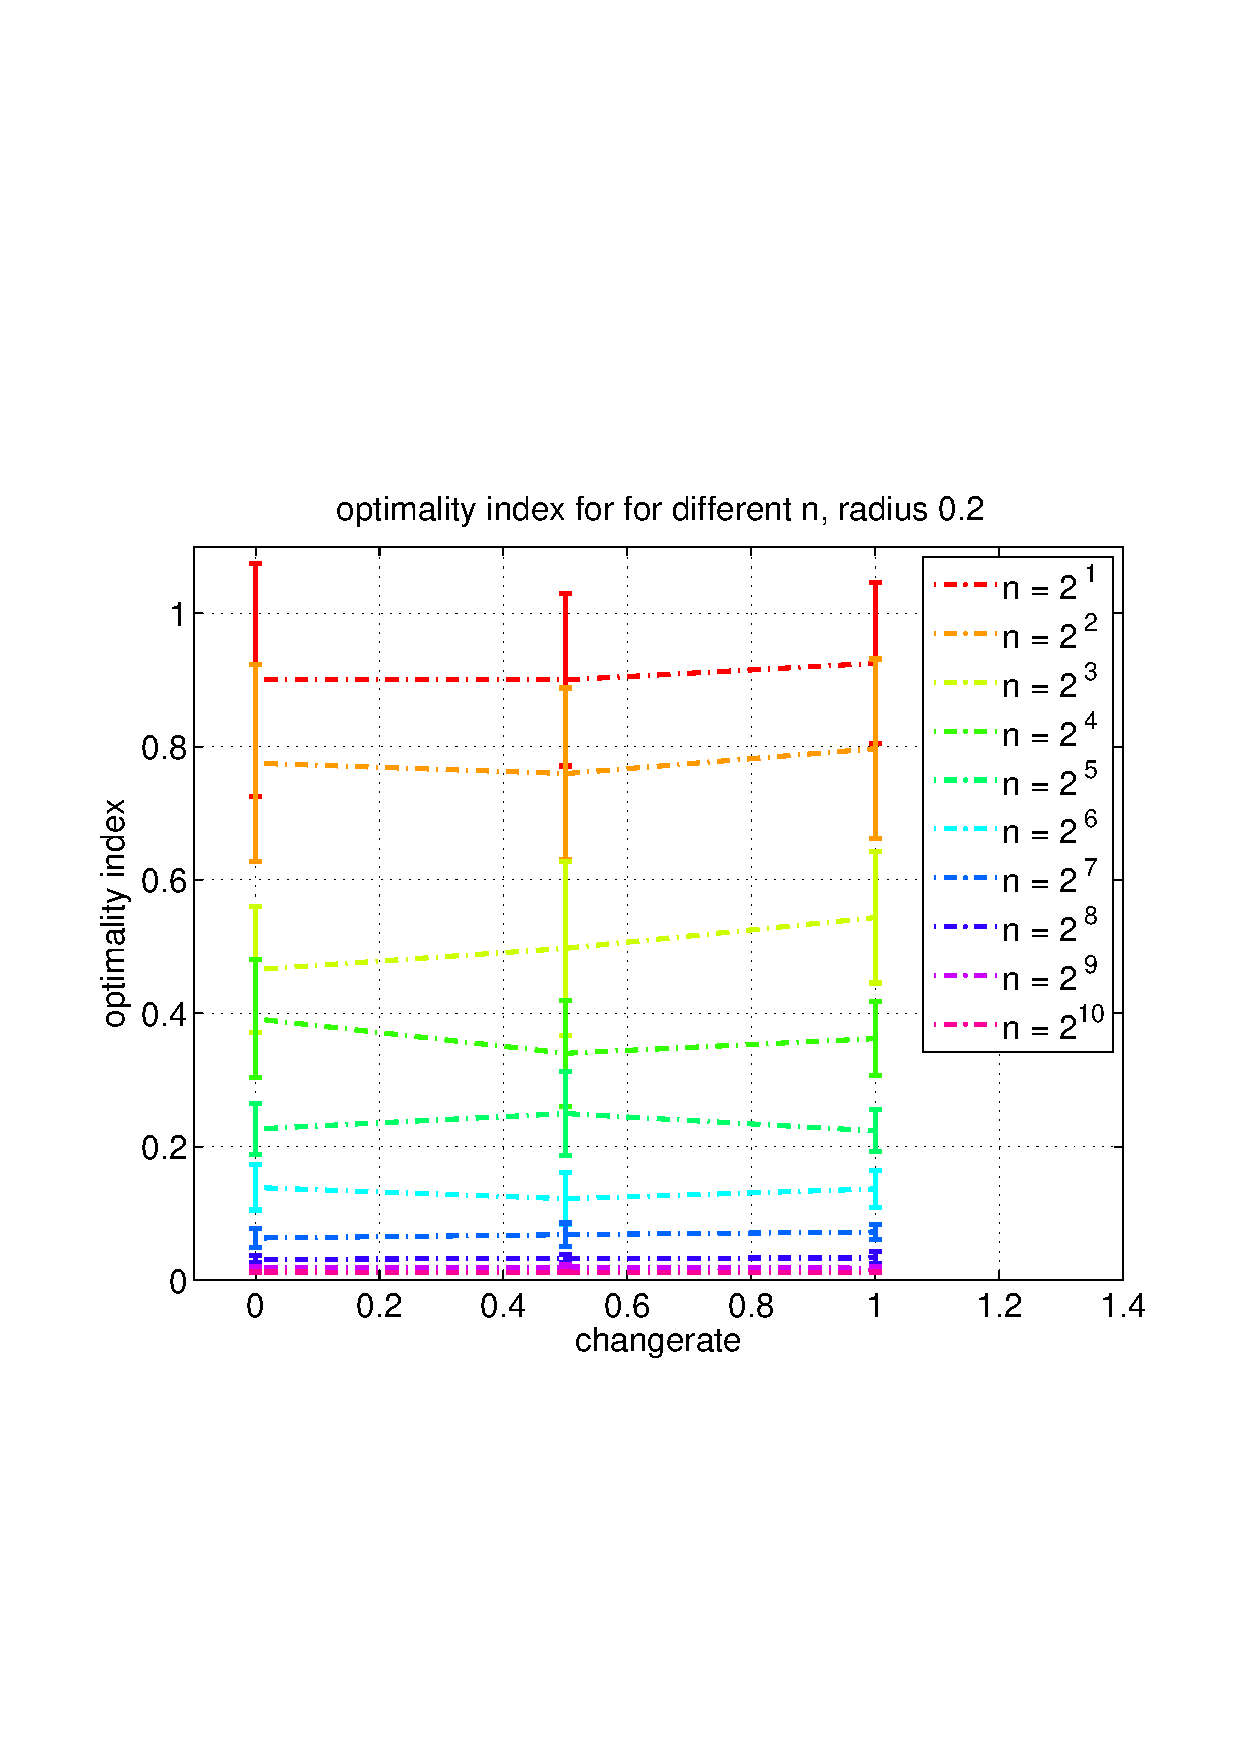
\includegraphics[width=\linewidth]{../../code/data/2014_12_12_00_55_41/figure_8}
\end{figure}
\begin{figure}
	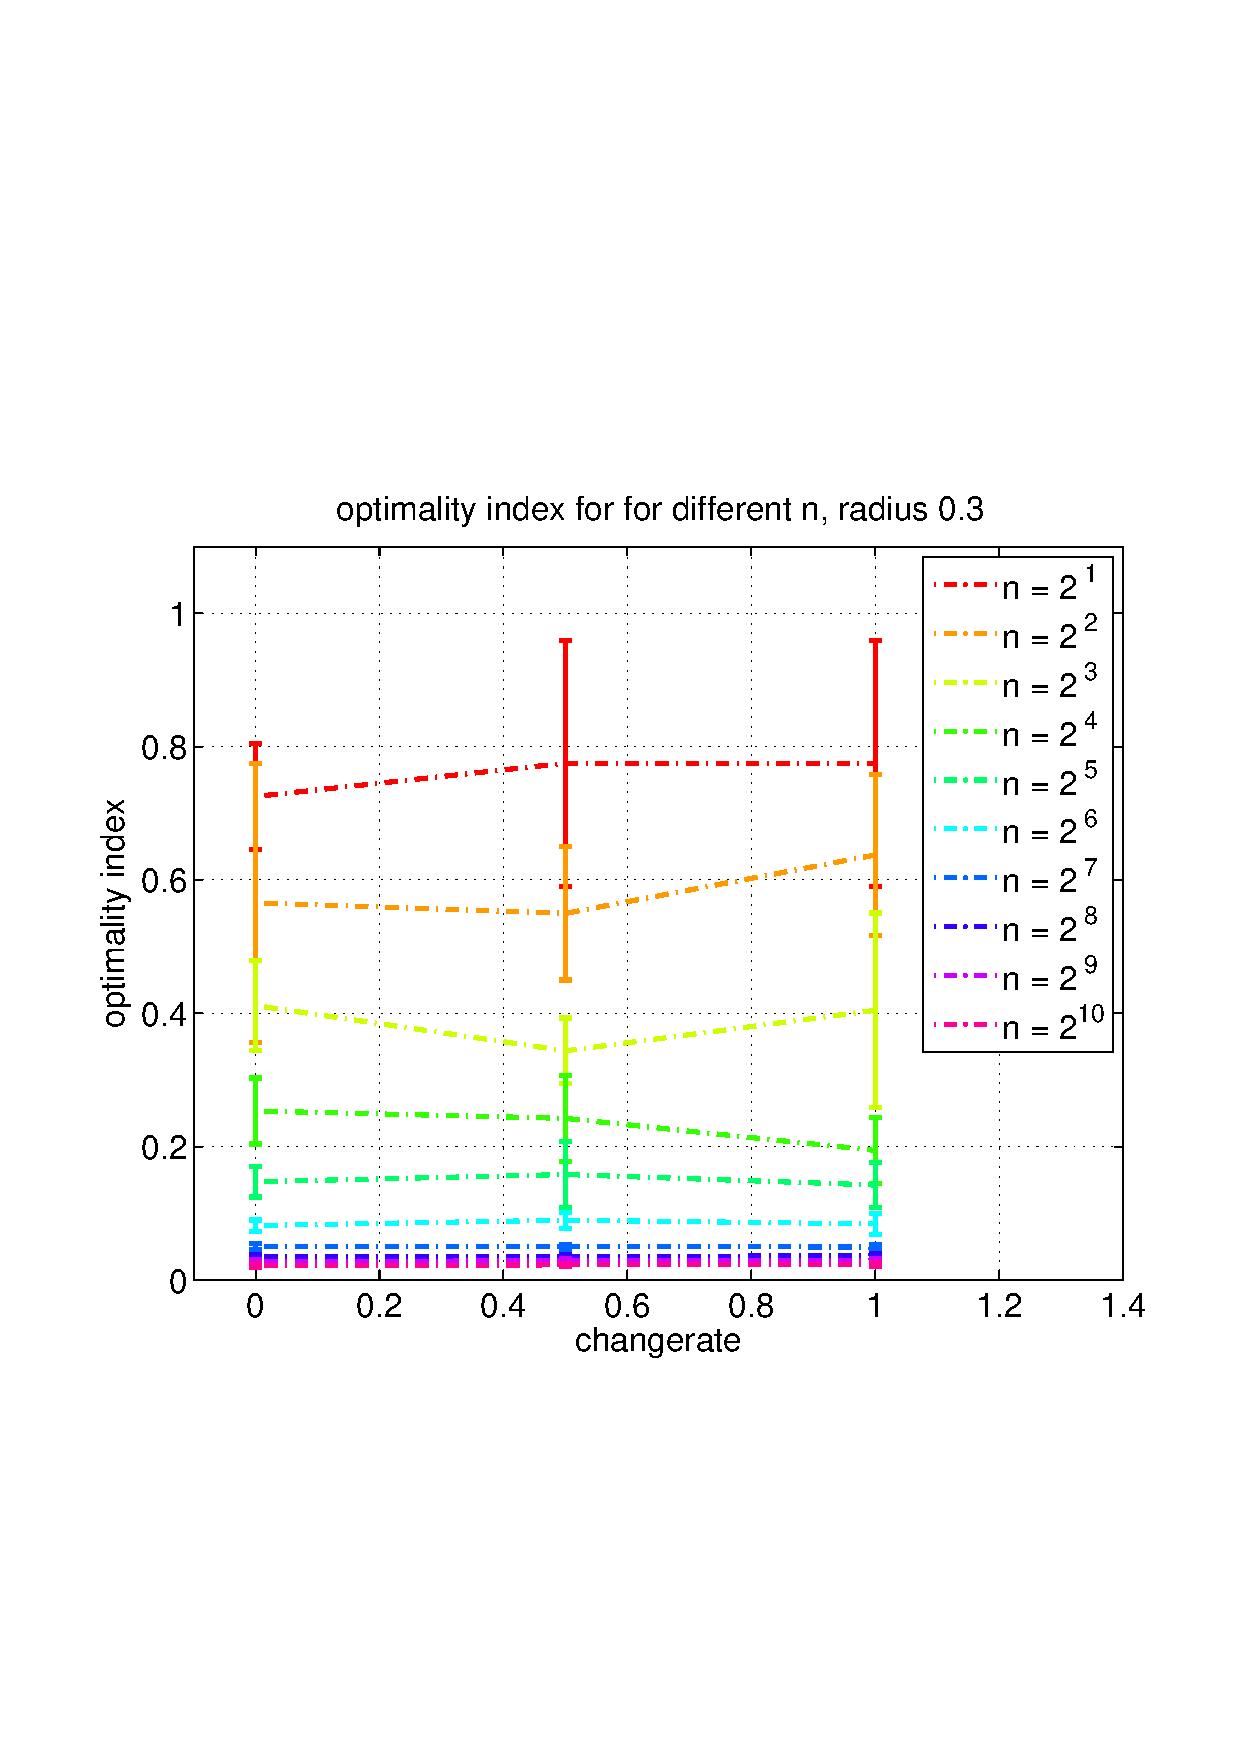
\includegraphics[width=\linewidth]{../../code/data/2014_12_12_00_55_41/figure_9}
\end{figure}
\begin{figure}
	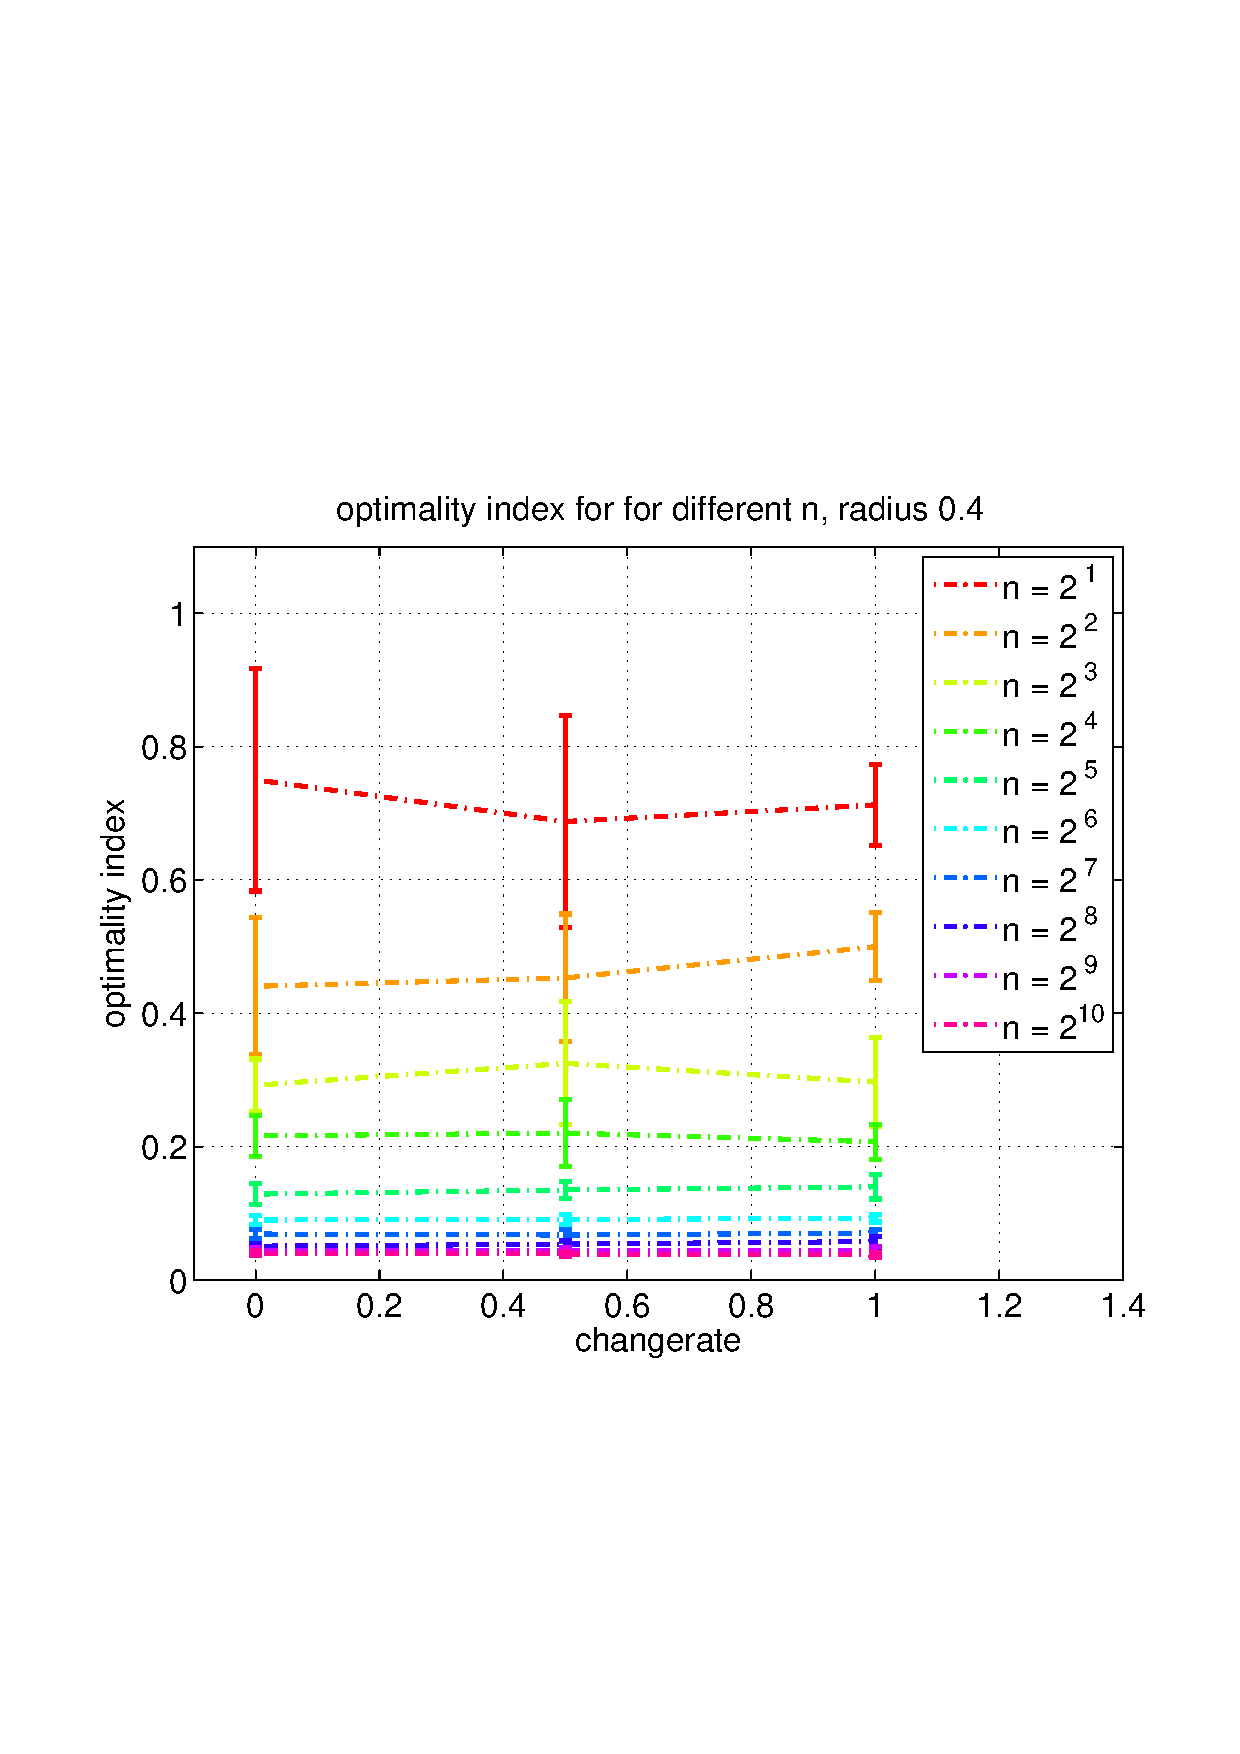
\includegraphics[width=\linewidth]{../../code/data/2014_12_12_00_55_41/figure_10}
\end{figure}
\begin{figure}
	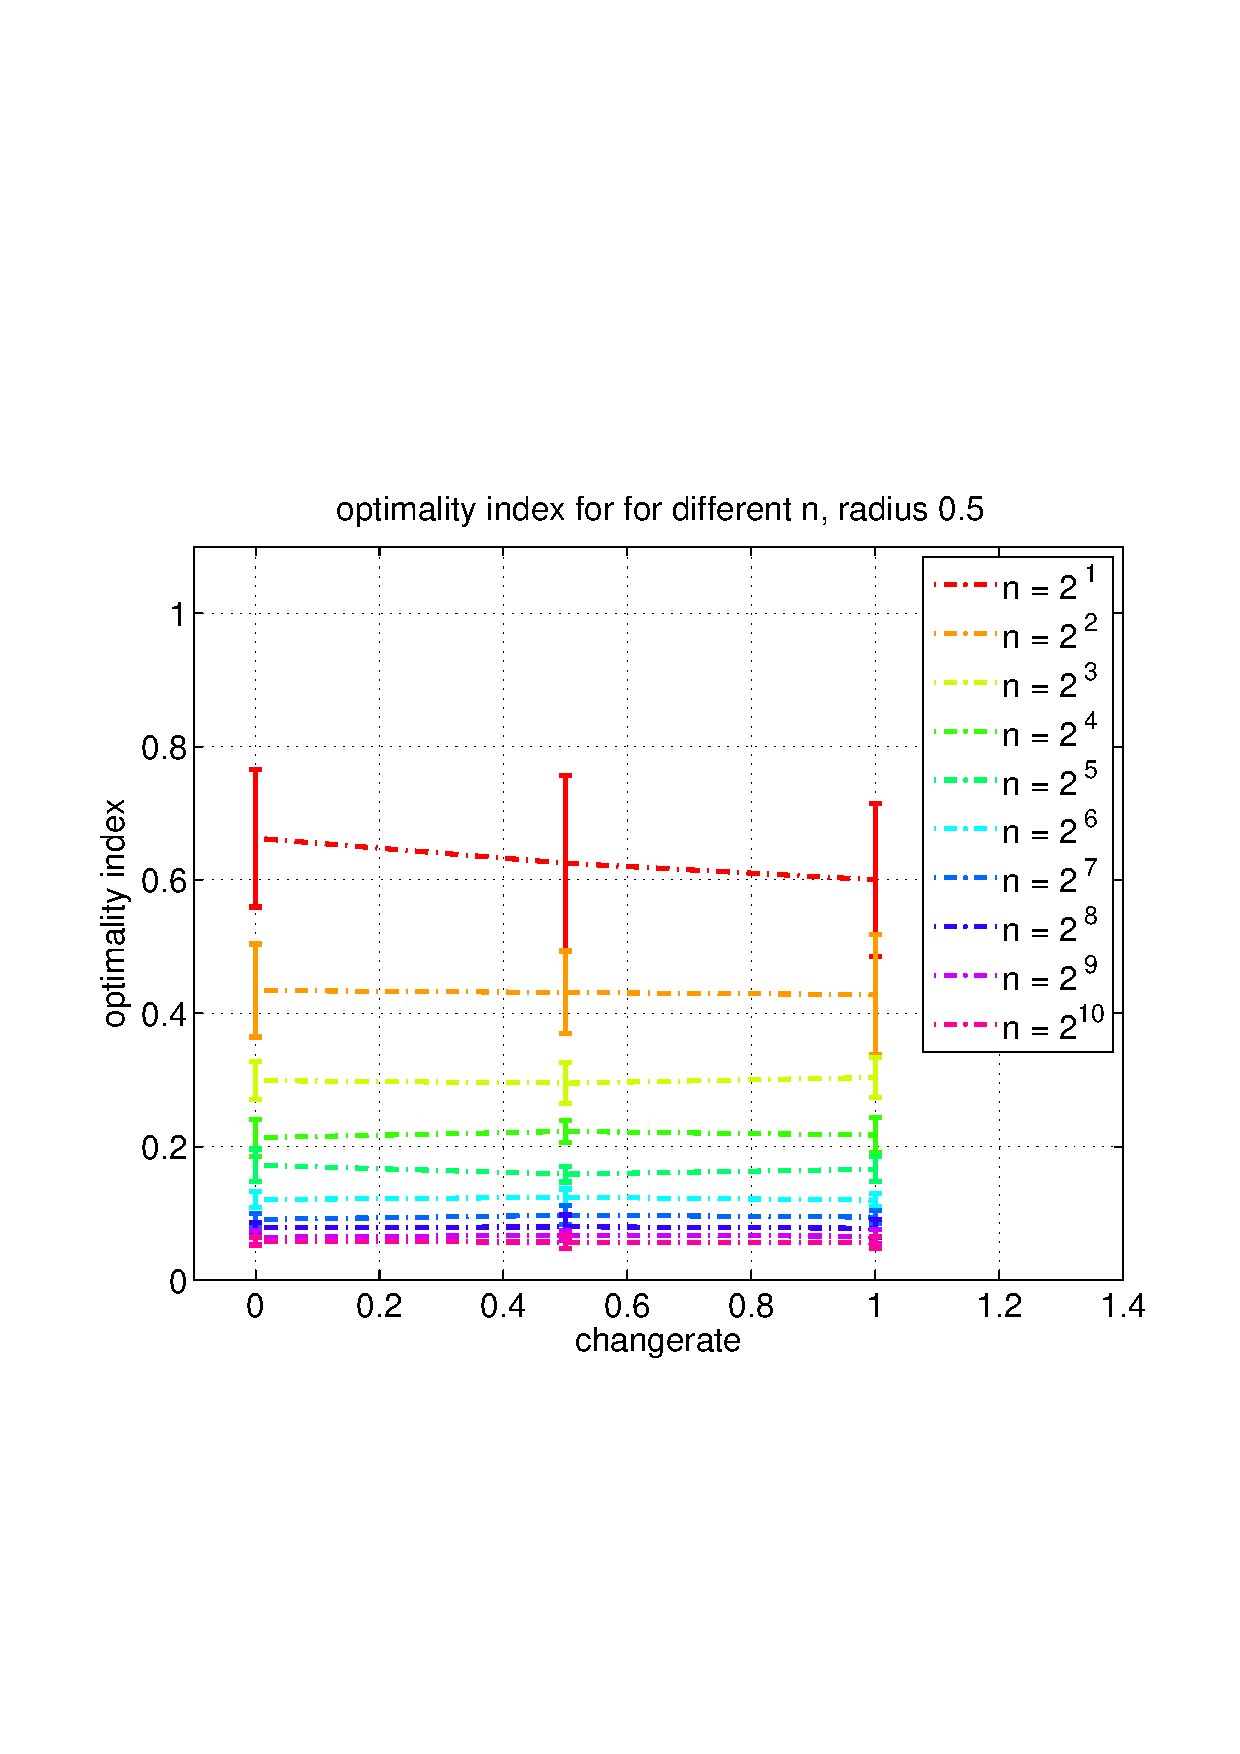
\includegraphics[width=\linewidth]{../../code/data/2014_12_12_00_55_41/figure_11}
\end{figure}
\begin{figure}
	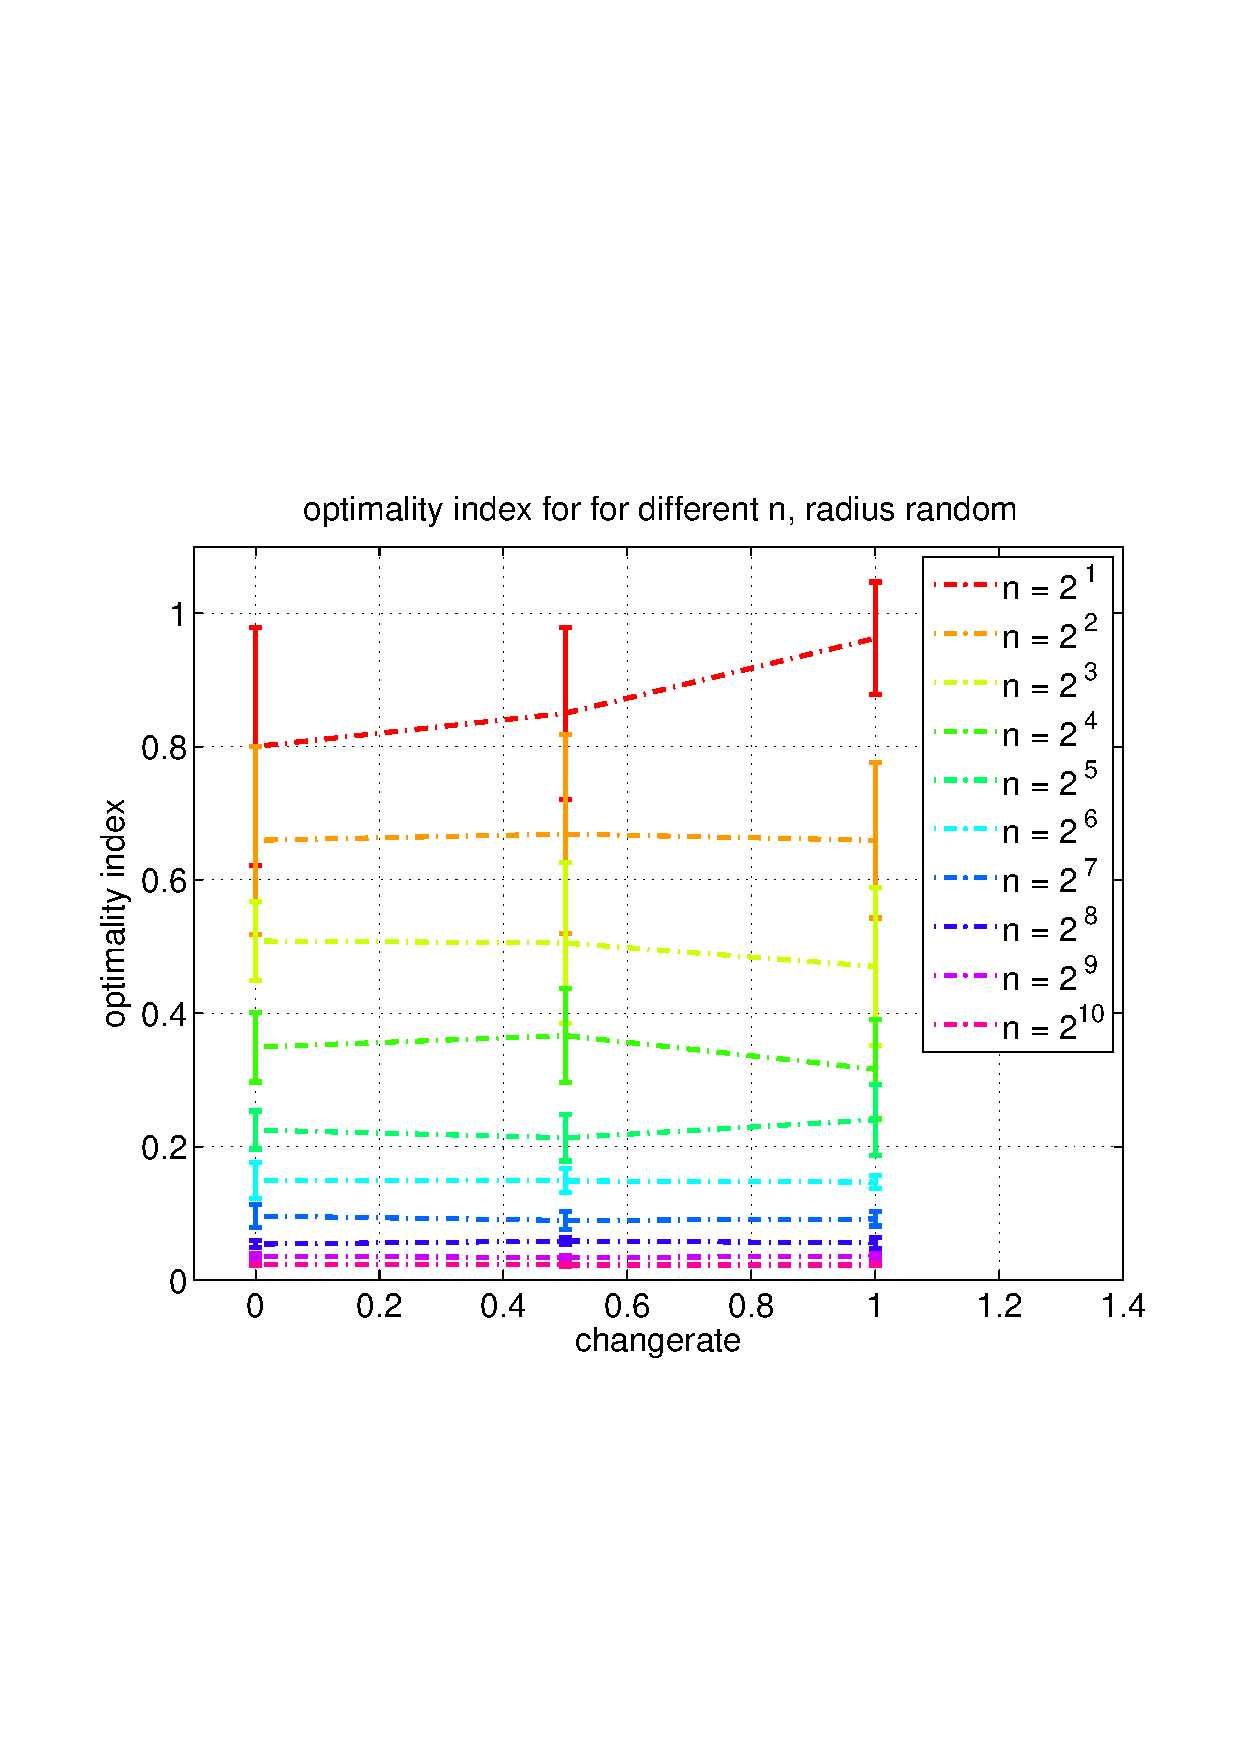
\includegraphics[width=\linewidth]{../../code/data/2014_12_12_00_55_41/figure_12}
\end{figure}
\begin{figure}
	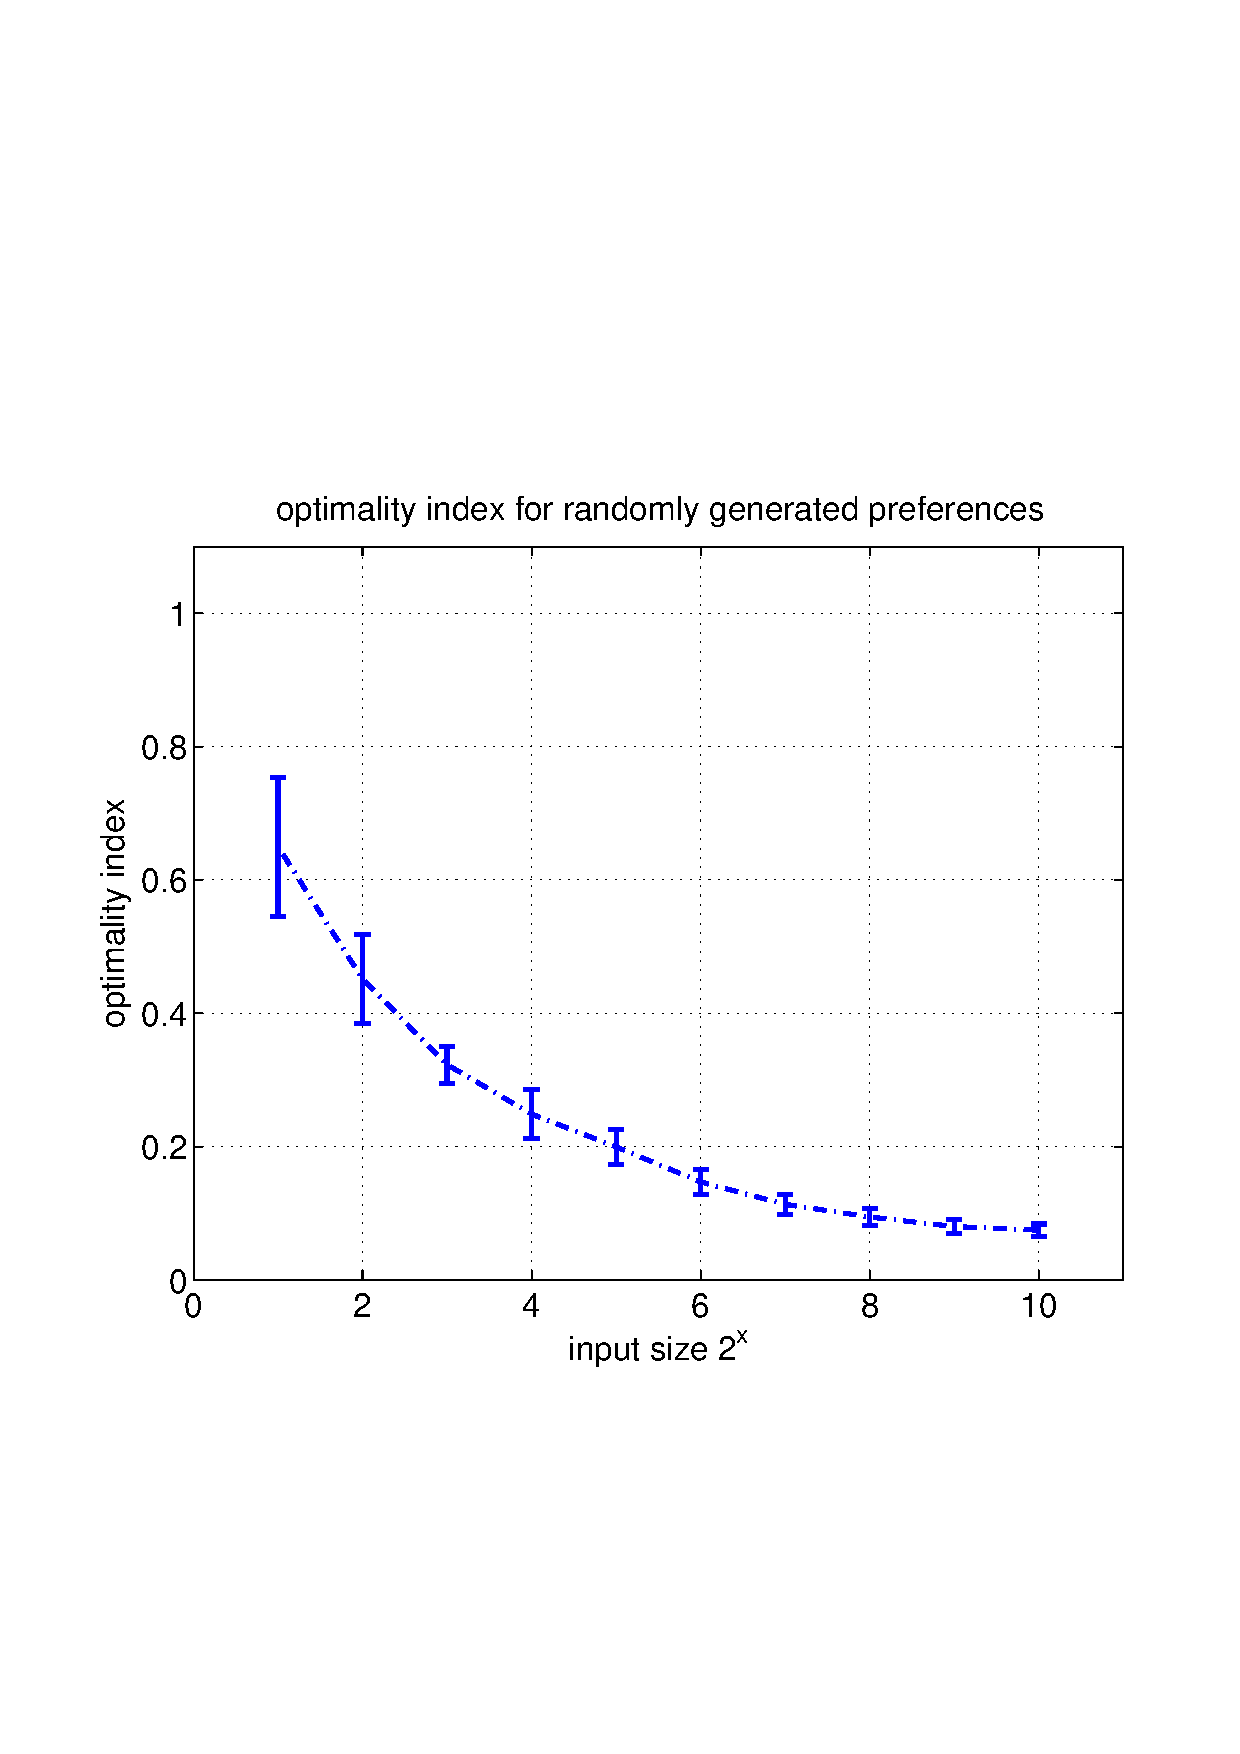
\includegraphics[width=\linewidth]{../../code/data/2014_12_12_00_55_41/figure_14}
\end{figure}


\end{document}  



 
